
\documentclass[12pt,a4paper,titlepage]{report}
%\documentclass[a4paper,12pt]{article}
\usepackage[utf8x]{inputenc}
\usepackage{amsfonts}
\usepackage{fancyhdr}
\usepackage{titlesec}
\usepackage{tocloft}
\usepackage{listings}
\usepackage[T1]{fontenc}
\usepackage{ascii}
\usepackage{graphicx}
\usepackage{pifont}
\usepackage{float}
\usepackage{sidecap}
\usepackage{wrapfig}
\usepackage{titletoc}
\usepackage{tocloft}
\usepackage[nottoc]{tocbibind}
\usepackage{afterpage}
%\usepackage[right=25mm,left=35mm,top=25mm,bottom=25mm]{geometry}
\usepackage[parfill]{parskip}
\usepackage{comment} 
%\usepackage[a4paper]{geometry}
\usepackage[numbers]{natbib}
\usepackage[right=0.75in,left=1in,top=0.75in,bottom=0.75in]{geometry}

\usepackage{balance}
\usepackage[table]{xcolor}
\usepackage{color}
\usepackage{amsmath}
%\usepackage[intlimits]{amsmath}
\usepackage{leftidx}
\usepackage[inference,shorthand]{semantic}
\usepackage{bm}
\usepackage{booktabs}
\usepackage{array}
\usepackage{tikz}
\usepackage[]{caption}
\usetikzlibrary{mindmap,trees}
\usepackage[UKenglish]{datetime}
\usepackage{acronym}
\usepackage{comment}
\usepackage[]{algorithm2e}
\usepackage{algorithmic}
\usepackage{subcaption}
%\usepackage[colorlinks=true,linkcolor=black]{hyperref}

\newcommand{\head}[1]{\textnormal{\textbf{#1}}}
\newcommand{\normal}[1]{\multicolumn{1}{l}{#1}}
\newcommand{\hilight}[1]{\colorbox{yellow}{#1}}	
\addtocontents{toc}{\protect\renewcommand{\protect\cftchapleader}{\bfseries\protect\cftdotfill{\protect\cftdotsep}}}
\newenvironment{cmd}{\fontfamily{ascii}\footnotesize\selectfont}{}
\setcounter{secnumdepth}{3}
\setcounter{tocdepth}{3}

%\titleformat{\chapter}[hang]{\huge}{\thechapter}{1em}{}
%\titlespacing{\chapter}{0pt}{0pt}{1cm}

\titleformat{\chapter}[hang] 
{\normalfont\huge\bfseries}{\chaptertitlename\ \thechapter:}{1em}{} 

\pagestyle{fancy}
%\fancyhead{}
%\fancyfoot{}


\fancyhead[LE,RO]{\slshape \rightmark}
\fancyhead[LO,RE]{\slshape \leftmark}
\fancyfoot[C]{\thepage}
%\headrulewidth 0.4pt
%\footrulewidth 0 pt

\setlength{\headheight}{18pt}
\addtolength{\textwidth}{1.0cm}
\addtolength{\hoffset}{-1cm}

%\fancyfoot[C]{\thepage}
\renewcommand{\headrulewidth}{1.2pt} 
%\renewcommand{\chaptername}{}

%___________________________________________________________________________%%%%
\begin{comment}

%%%%%%%%%%%%% Preparing Oerview Diagrams %%%%%%%%%%%%%%%%%%%%%%%%
%%%%%%%%%%

\usetikzlibrary{shadows,arrows,positioning}

% Define the layers to draw the diagram
\pgfdeclarelayer{background}
\pgfdeclarelayer{foreground}
\pgfsetlayers{background,main,foreground}

% Define block styles
\tikzstyle{materia}=[draw, fill=yellow!15, text width=10.0em, text centered,
  minimum height=7.5em,drop shadow]
\tikzstyle{practica} = [materia, text width=10em, minimum width=12em,%(minimum width=2em) change the width of the yellow block
  minimum height=5em, rounded corners, drop shadow]%(minimum height=5em) change the height of the yellow block
\tikzstyle{texto} = [above, text width=15em, text centered]
\tikzstyle{linepart} = [draw, thick, color=black!60, -latex', dashed]
\tikzstyle{line} = [draw, thick, color=black!240, -latex']
\tikzstyle{ur}=[draw, text centered, minimum height=0.01em]
\usetikzlibrary{fadings}
\usetikzlibrary{decorations}
\usepgflibrary{decorations.pathmorphing}

\tikzfading[name=fade out, inner color=transparent!0,
  outer color=transparent!100]

% Define distances for bordering
\newcommand{\blockdist}{1.3}
\newcommand{\edgedist}{1.5}

%\newcommand{\etape}[2]{node (p#1) [etape]
 % {#2}}

\newcommand{\Step}[2]{node (p#1) [practica]
  {\\{ \Large\textit{#2}}}}

% Draw background
\newcommand{\background}[5]{%

  \begin{pgfonlayer}{background}

    % Left-top corner of the background rectangle
    \path (#1.west |- #2.north)+(-0.3,0.5) node (a1) {};
    % Right-bottom corner of the background rectanle
    \path (#3.east |- #4.south)+(+0.3,-0.5) node (a2) {};


    % Draw the background
   \path[fill=gray!30,rounded corners, draw=black!50, dashed]
     (-4,-8.5) rectangle (1,3);

   \path[fill= gray!30,rounded corners, draw=black!50, dashed]
     (1.8,-11.6) rectangle (6.8,-3.5);

%%%%%%%%%%%%%
 %\fill[yellow!10!black] (-1,1) rectangle (4,3);
    %\fill[yellow] (-4,-5.2) rectangle (4,1);
   %\fill[inner color=blue!50!,outer color=blue!10!black] (4.7,-5.2) rectangle (12.5,1);
%%%%%%%%%%%%%%%%%%%%%%%%%%

 \path (a1.east |- a1.south)+(3.5,0.5) node (u1)[texto]
      { \LARGE\textit{ #5}};

      \path (#3.east |- #2.north)+(0,0.25)--(#1.west |- #2.north) node[midway] (#5-n) {};
      \path (#3.east |- #2.south)+(0,-0.35)--(#1.west |- #2.south) node[midway] (#5-s) {};
      \path (#3.east |- #2.north)+(0.7,0)--(#3.east |- #4.south) node[midway] (#5-w) {};

  \end{pgfonlayer}}

\newcommand{\transreceptor}[3]{%
  \path [linepart] (#1.east) -- node [center]
    {\large #2} (#3);}


\end{comment}

%___________________________________________________________________________%%%%

\usetikzlibrary{shadows,arrows,positioning}
% Define the layers to draw the diagram
\pgfdeclarelayer{background}
\pgfdeclarelayer{foreground}
\pgfsetlayers{background,main,foreground}

% Define block styles
\tikzstyle{materia}=[draw, fill=yellow!40, text width=10.0em, text centered,
  minimum height=7.5em,drop shadow]
\tikzstyle{practica} = [materia, text width=8em, minimum width=6em,
  minimum height=4em, rounded corners, drop shadow]
\tikzstyle{texto} = [above, text width=10em, text centered]
\tikzstyle{linepart} = [draw, thick, color=black!60, -latex', dashed]
\tikzstyle{line} = [draw, thick, color=black!50, -latex']
\tikzstyle{ur}=[draw, thick, text centered, minimum height=0.01em]
\usetikzlibrary{fadings}
\usetikzlibrary{decorations}
\usepgflibrary{decorations.pathmorphing}

\tikzfading[name=fade out, inner color=transparent!0,
  outer color=transparent!100]
\tikzset{>=latex}
% Define distances for bordering
\newcommand{\blockdist}{1.3}
\newcommand{\edgedist}{1.5}



%++++++++++++++++++++++++++++++++++++++++
%\newcommand{\practica}[2]{node (p#1) [practica]
  %{Pr\'actica #1\\{\scriptsize\textit{#2}}}}

\newcommand{\Step}[2]{node (p#1) [practica]
  {\\{ \Large\textit{#2}}}}

%++++++++++++++++++++++++++++++++++++++++


% Draw background
\newcommand{\background}[5]{%
  \begin{pgfonlayer}{background}
    % Left-top corner of the background rectangle
    \path (#1.west |- #2.north)+(-0.3,0.9) node (a1) {};
    % Right-bottom corner of the background rectanle
    \path (#3.east |- #4.south)+(+0.5,-0.35) node (a2) {};

%++++++++++++++++++++Two backgrounds++++++++++++++++++++

    % Draw the background
    \path[fill=gray!20,rounded corners, draw=black!50, dashed]
      (a1) rectangle (a2);

     %  \path[fill=blue!20,rounded corners, draw=black!50, dashed]
     %(-4,-5.2) rectangle (4,1);

%++++++++++++++++++++++++++++++++++++++++



 \path (a1.east |- a1.south)+(1.9,-0.57) node (u1)[texto]%place of the text above the diagram
      {\Large\textit{ #5}};

      \path (#3.east |- #2.north)+(0,0.25)--(#1.west |- #2.north) node[midway] (#5-n) {};
      \path (#3.east |- #2.south)+(0,-0.35)--(#1.west |- #2.south) node[midway] (#5-s) {};
      \path (#3.east |- #2.north)+(0.7,0)--(#3.east |- #4.south) node[midway] (#5-w) {};
  \end{pgfonlayer}}

\newcommand{\transreceptor}[3]{%
  \path [linepart] (#1.east) -- node [above]
    {\scriptsize #2} (#3);}






%%%%%%%%%%%%%%%%%% BEGING Document %%%%%%%%%%%

\begin{document}



%%%%%%%%%
%%%%%%%%%%%%%%%%%%%% Title page %%%%%%%%%%%%%
%%%%%%%%%

\begin{titlepage}
\vspace*{\fill} % Vertical Align
\begin{center}




%	LOGO SECTION
%----------------------------------------------------------------------------------------


\includegraphics[width=0.4\textwidth]{logo.jpg}\\[2.4cm] 

%----------------------------------------------------------------------------------------



% Title
\textbf{\LARGE Platform for Microrobot Navigation} \\ [1.5cm]


% Author and date
\textbf{\LARGE Nafiseh Vahabi} \\ [1.3cm]


% Report title
\textbf{\normalsize A thesis submitted in partial fulfilment of the requirements for the degree of } \\ [0.2cm]
\textbf{\normalsize MRes in Medical Robotics and Image Guided Intervention and for the Diploma of}\\ [0.2cm]
\textbf{\normalsize  Imperial College}\\ [2.3cm]


\textbf{\LARGE Imperial College London} \\ [0.6cm]
\textbf{\large Department of Surgery and Cancer} \\ [1.90cm]

\newdateformat{UKvardate}{%
 \monthname[\THEMONTH], \THEYEAR}
\UKvardate
\textbf{\large \today} \\ [1.9cm]

% Examiner details
\textbf{\large  Dr. Henry Ip} \\ [0.3cm]
\textbf{\large  Dr. Vincenzo Curto} \\ [0.3cm]
\textbf{\large Prof. Guang-Zhong Yang} \\ [1.5cm]




\end{center}
\vspace*{\fill}
\end{titlepage}

%%%%%%%%%
%%%%%%%%%%%%%%%%%%%%END Title page %%%%%%%%%%%%%
%%%%%%%%%

\pagenumbering{roman}

%\section{Acknowledgements}
%\addcontentsline{toc}{chapter}{\numberline{}Acknowledgements}
%\pagenumbering{roman}
\setcounter{page}{1}
\thispagestyle{plain}
\chapter*{Acknowledgements}

First and foremost, I wish to express my sincere thanks to my supervisor Prof. Yang for his valuable guidance 
and supervision all through my MRes course.

\paragraph{}
My special gratitude to my supervisors Dr. Henry Ip and Dr.Vincenzo Curto for their assistance 
and suggestions all throughout of the project. Thanks for helping me to improve my final presentation, 
reading the draft of my thesis and providing me with your comment and feedback.

\paragraph{}
I would like to thank Dr. Ebubekir Avci for helping me to take images of my fabricated structures with 
Scanning Electron Microscope.

\paragraph{}
I would like to thank the course leader Dr. Daniel Elson for all his organisation and arrangements
 for the MRes students to make the course enjoyable.

\paragraph{}
  I am most grateful to my husband Ali for all his love, support and encouragements during 
my study. Thanks for advising me throughout the project, for your patient to proofreading my thesis
 and most importantly your care for our children during this pressured time. This thesis would not 
have been possible without you.

\paragraph{}
  I would like to thanks to my daughter Parmin and my son Ario for always giving me their love and joy.

\paragraph{}
Finally, my special thanks to my parents and my brother for their encouragement and support during the project.






\pagebreak


\renewcommand{\cftsecleader}{\cftdotfill{\cftdotsep}}
\tableofcontents
%\setcounter{secnumdepth}{2}
%\setcounter{page}{1}

\pagebreak



%\addcontentsline{toc}{chapter}{\numberline{}List of Figures}
\setcounter{page}{3}
%\thispagestyle{plain}
\listoffigures
%\chapter*{List of Figures}
\pagebreak



%\addcontentsline{toc}{chapter}{\numberline{}List of Tables}
\setcounter{page}{4}
%\thispagestyle{plain}
\listoftables
%\chapter*{List of Tables}
\pagebreak


%%%%%%%%%%%%%%%%% List of ACronyms %%%%%%%%%%%%%%%

\setcounter{page}{5}
\chapter*{List of Acronyms}

\begin{acronym}
\addcontentsline{toc}{chapter}{\numberline{}List of Acronyms}
\acro{SBT}{Slender Body Theory}
\acro{FBMS}{Fixed-beam Moving-sample}
\acro{gwl}{General Writting Language}
\acro{MPC}{Magnetic Polymer Composite}
\acro{MBFS}{Moving-beam Fixed-sample}
\acro{RFT}{Resistive Force Theory}
\acro{RSM}{Regularized Stokeslet Method}
\acro{SEM}{Scanning Electron Microscope}
\acro{stl}{STereoLithography}



\end{acronym}

\pagebreak

%------------------------------------------- Abstract -------------------------------------

\begin{abstract}
%\addcontentsline{toc}{chapter}{\numberline{}Abstract}
%abstract

Structures and functions of microorganisms were made them suitable reference to design
 microrobots. Flagellar propulsion of microorganism such as E.coli is used as an efficient approach for 
modelling micro swimmers locomotion method in low Reynolds number regime. Microrobots were 
demonstrated precise and controllable movements under low strength magnetic field. A system with 
a size of bacteria, capable to swim in viscous fluid in a controllable manner was satisfied basic principles
 for performing delicate tasks such as targeted drug delivery in medical application. Furthermore 
microrobots were advantaged from fabrications technology to make them biocompatible. 
In this study we reviewed a range of bio mimetic microrobots in terms of their design, fabrication, propulsion 
method in the fluid environment. 
The key characteristics of the helical shape microswimmers were optimised and the new design of helical
 microrobot is presented. The new design is demonstrated the microrobot with the variable pitch that is
 satisfied the fabrication requirement. 

Three propulsion methods; Resistive Force Theory, Regularised Stokeslet Method 
and Slender Body Theory were implemented. The last two methods have not used before
 for remotely controlled microrobots. We provide the simulation platform for the 
swimming microrobot in a high viscose fluid. The simulation algorithm takes a desired velocity of microrobot
and calculate the electric current is required to generate a dynamic magnetic field.





%\pagenumbering{roman}
\setcounter{page}{6}
\thispagestyle{plain}

\end{abstract}

%-------------------------------------------END Abstract -------------------------------------

\pagenumbering{arabic}

%%%%%%%%%
%%%%%%%%%%%%%%%%%%%% Introduction %%%%%%%%%%%%%
%%%%%%%%%

\chapter{Introduction}


Robotic surgery has demonstrable advantages such as reducing pain and discomfort and 
minimising scaring after invasive surgery. As robotic technology continues to move towards miniaturisation, the idea of using
a microrobot for medical applications such as cardiovascular  surgery, also becomes more attractive~\citep{phil2013robotics}
The potential applications of a microrobot can be classified into two main categories; in vivo and in vitro applications.
Some in vivo examples are drug delivery, delivery of hyperthermia for cancer treatment and ablation  of material.
In vitro applications can be microfluid control and cell characterisation and manipulation~\citep{edd2003biomimetic}.  


\paragraph{}

Magnetically actuated helical microswimmers have been reported as a safe microdevice for biomedical applications
~\citep{peyer2013magnetic}. However, there are number of challenges such as the issue of biocompatibility and the material 
used to make a microrobot, which needs to be considered carefully for in vivo application\citep{qiu2014noncytotoxic}.
Research into swimming microrobots has identified two primary difficulties, namely the power source and a suitable locomotion method, because
there are many cells, proteins and fibres in biofluid that prevent the motion of the microrobots~\citep{peyer2013bio}. 
The extremely small size of the microrobot and the
complex biofluid environment makes the design aspect very challenging.   
Furthermore, the design of a microrobot will depend on its application and the desired task to be performed.
Artificial bacteria flagella is a popular microrobot inspired by nature~\citep{qiu2014noncytotoxic}. 
They have helical shape, are composed of magnetic material and are capable to mimic three-dimensional 
motion of the bacteria in a high viscous fluid.

 


\paragraph{}
The motivation for developing a simulation platform for microroswimmers navigation is raised to analyse
 their characteristic and behaviour under low magnetic field. A few numbers of parameters 
has a key role on designing the helical shape microswimmer. The simulation
challenge can be divided into two main parts; propulsion mechanism of the microrobot and actuation method. The
popular method, \ac*{RFT}, describes the motion of the helix object in a low number regime 
is applied by most helical microswimmers\rq{}s algorithms\citep{qiu2014noncytotoxic}. In this
project, we studied two more propulsion methods for the remotely controlled helical microswimmers
 in a dynamic magnetic field, \ac*{RSM} and \ac*{SBT}. An actuation method of a magnetic  microrobot 
can be either force driven or
torque driven~\citep{qiunanohelices}. Fabrication of a microdevice has been a considerable challenge 
for some time ~\citep{qiunanohelices}, which has now been
overcome by fabrication methods such as 3D laser lithograph.



\paragraph{}
In summary, a part of the algorithm developed for the propulsion mechanism of the microswimmers
and their actuation technique was based on \citeauthor{mahoney2011velocity}\rq{}s research. Two new 
propulsion methods for the helical microswimmers were used in the \citeauthor{rodenborn2013propulsion}\rq{}s
work. This involved a reversible speed-variable motor such as a micro metal gear motor being used to rotate 
the microswimmer. In this study, these two propulsion mechanisms were applied to the microswimmers that 
are then controlled remotely by a magnetic field. Therefore, the algorithm has taken the desired translational
velocity as an input and produced the rotational velocity as an output. By knowing the rotational velocity, 
we will be able to compute the electric current required to produce the desired translational velocity. 
In addition, the new design is developed and printed for the helix using a variable pitch
in the helix design rather than a constant pitch to satisfy 
 the fabrication process. 



%%%%%%%%%%%%
%%%%%%%%%%%%%%%%% OVERVIEW DIAGRAM %%%%%%%%%%%%%%%%%%
%%%%%%%%%%%%


\begin{figure}
        \centering
        \begin{subfigure}[b]{1.0\textwidth}
                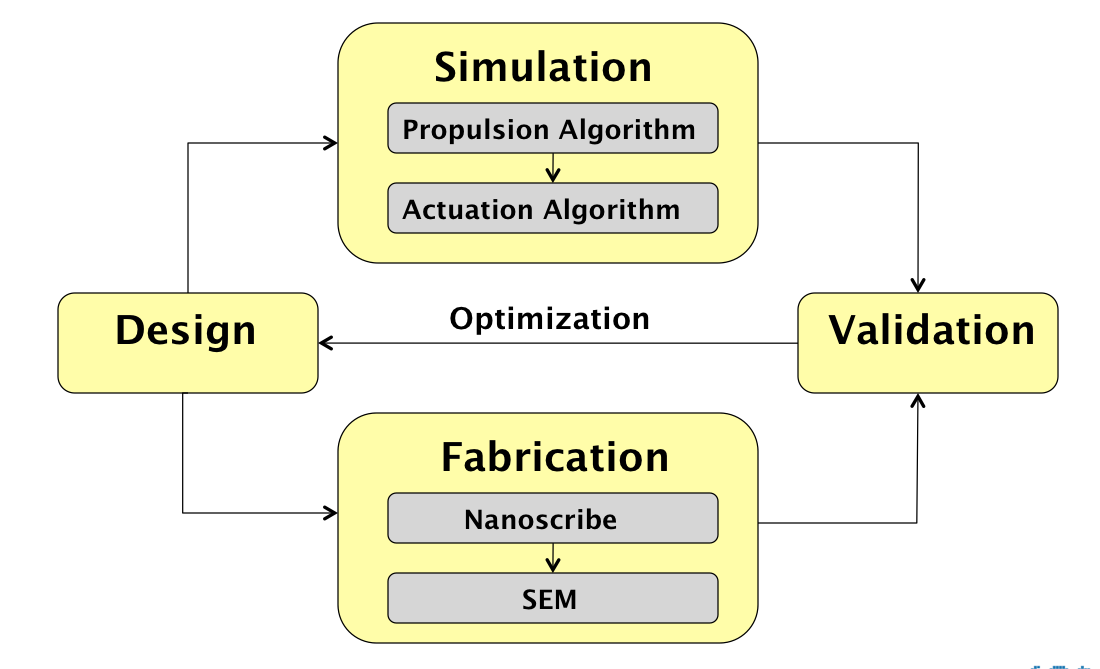
\includegraphics[width=\textwidth]{overview_Dig1}
                \caption{Simulation framework}
                \label{simulation}
        \end{subfigure}~~ 

    
      
        \caption[Simulation framework]{Simulation framework. (a) The framework consists of the three inset coils,
a fluid bux with a microhelix inside (b).}\label{Simulation framework}

   %add desired spacing between images, e. g. ~, \quad, \qquad, \hfill etc.
          %(or a blank line to force the subfigure onto a new line)
       
         %add desired spacing between images, e. g. ~, \quad, \qquad, \hfill etc.
          %(or a blank line to force the subfigure onto a new line)

\end{figure}











\begin{comment}
\begin{figure}
\centering
\begin{tikzpicture}[<->,scale=1.25,transform shape]

  % Draw diagram elements
  \path \Step{1}{Propulsion Algorithm};
  \path (p1.south)+(0.0,-2.0) \Step{2}{Actuation Algorithm};

  \path (p2.south)+(0.0,-3.5) \Step{3}{Nanoscribe};
  \path (p3.south)+(0.0,-2.0) \Step{4}{SEM};
   \path (p4.east)+(3.0,5.5) \Step{6}{Optimisation};
  \path (p6.west)+(-8.0,0.00) \Step{5}{Design};


  %\path (p4.east)+(5.0,0.0) \practica{7}{Calculate forward and inverse kinematic};
  %\path (p5.east)+(5.0,0.0) \practica{8}{Design feedback control mechanics};

  %\path (p5.south)+(3.5,-2.0) \practica{9}{Integrating e-AR and robot};
  %\path (p9.south)+(0.0,-1.5) \practica{10}{Laparoscopy Robot};
%\draw [>=stealth,red] (0,.6) -- +(1,0);
%\draw [blue] (0,.3) -- +(1,0);
%\draw (0,0) -- +(1,0);

  % Draw arrows between elements
  \path [line] (p1.south) -- node [above] {} (p2);
  \path [line] (p3.south) -- node [above] {} (p4);
 \path [line] (p5.north) -- node [above] {} (p1);
  \path [line] (p5.south) -- node [above] {} (p3);

 \path [line] (p4.east) -- node [above] {} (p6);
  \path [line] (p2.east) -- node [above] {} (p6);

  %\path [line] (p5.south) -- node [above] {} (p9);
  %\path [line] (p8.south) -- node [above] {} (p9);
 % \path [line] (p9.south) -- node [above] {} (p10);



  \background{p1}{p1}{p2}{p2}{Simulation }
  \background{p3}{p3}{p4}{p4}{Fabrication}

  

 % \path [line] (p5.south) -- node [above] {} (bk3-n);
 % \path [line] (bk3-s) -- node [above] {} (p8);
 % \path [line] (bk3-s) -- node [above] {} (p9);
  %\path (bk1-e)+(+6.0,0) node (ur1)[ur] {};
 % \path (bk2-w)+(+6.0,0) node (ur2)[ur] {};
  %\path (bk3-w)+(+3.0,0) node (ur3)[ur] {};
% \transreceptor{bk1-e}{pre processing}{ur1};
 % \transreceptor{bk2-w}{Feature selection}{ur2};
  %\transreceptor{bk3-w}{classification}{ur3};


%%%%%%%%%%%%%% CHANGED%%%%%%%%%%%%%
\end{tikzpicture}									   %
\caption{System Architecture.}						   %
\label{System Architecture}										   %
\end{figure}										   %	
												   %
%%%%%%%%%%%%%% CHANGED%%%%%%%%%%%%%

\end{comment}

\paragraph{}


A literature review on the different aspects of microrobots is presented in chapter 1.
An overview of the main microrobot designs are summarised in the table \ref{Micro}.  
Section \ref{microDesign} demonstrates the details of the effective parameters on 
microrobot\rq{}s design and optimises them to characterise the new design for 
a helix shaped microrobot. The major part of this project involves studying, solving and 
implementing the simulation methods
 described in section \ref{simulation}.  
Whilst the mechanism of both methods are explained in the section \ref{microActuation}, we
only implemented the torque driven actuation method in this study. 
Section \ref{fabrication} presents a brief history of the fabrication techniques and section \ref{microFabric}
 describes the fabrication method applied in this study. Chapter 3 provided the results of this work in terms of both
simulation and fabrication. The key issues are discussed in chapter 4 and conclusion and potential
future work is described in chapter 5. An overview of the entire system is shown in diagram \ref{System Architecture}.














%%%%%%%%%
%%%%%%%%%%%%%%%%%%%% literature review %%%%%%%%%%%%%
%%%%%%%%%


\section{Literature review}
 


\subsection{Bioinspired microrobots}

One of the most challenging aspects of designing a robot on a very small scale such 
as a nanorobot is simplicity. The reason is, integration between various components
will become unfeasible on that
 scale if the design is complex. Hence the development of the nanorobot or even microrobot
 should be based on the essential functionality, avoiding any unnecessary components~\citep{gao2013bioinspired}.
By learning from nature and mimicking the structure of live organisms, the successful  
scientific applications were created~\citep{qiunanohelices}. In the following section a
 few examples of swimming microrobots that were imitated from nature will describe. 
 



\paragraph{Reynolds number}

To understand how micro organisms swim in a fluidic environment, it is essential to study their propulsion 
mechanism. In the fluidic regime the Reynold number (Re) has a substantial effect on a microdevice
locomotion~\citep{peyer2013magnetic}. The Reynolds number describes the ratio of the inertial forces versus viscous 
forces according the following formula;

\begin{equation}
  Re = \cfrac{UL\rho}{\mu}
\label{eq:4}
\end{equation}
 
Where $ U$ is velocity, $L$ is characteristic length, $\rho$ is the density and $\mu$ is viscosity of the fluid.






\subsubsection{Flagella style microrobots}

Helical flagella and cilia are two well-known microswimers in nature that have had their functionality employed 
for motion generation in artificial microrobots  (Figure~\ref{cilia}) ~\citep{gao2013bioinspired}. 



\begin{figure}
  \centering
    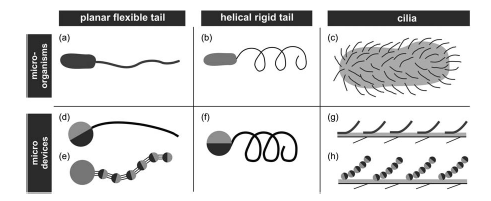
\includegraphics[width=0.9\textwidth]{cilia}
  \caption[Micro-structures and microdevices]{Micro-structures and microdevices. The illustration of both flagellum and cilia shapes and microdevices mimicked the flagellum and cilia 
structures~\citep{peyer2013bio}.}
	
  \label{cilia}
\end{figure}


 
\paragraph{}

%\begin{figure}
%  \centering
\begin{wrapfigure}{r}{0.5\textwidth}
  \begin{center}
    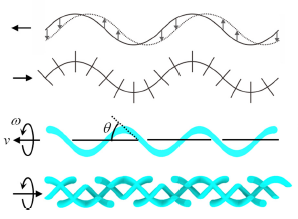
\includegraphics[width=0.5\textwidth]{10}
  \caption[Propulsion mechanism of mastigonemes flagellum]{ The propulsion mechanism of the smooth flagellum and a mastigonemes flagellum.
The propulsion direction of smooth flagellum (top design) is opposite of flagella\rq{}s propagation 
wave (second from the top). Their artificial design (blue structures) is based on 
their locomotion mechanism~\citep{gao2013bioinspired}.}
  \label{10}
\end{center}
\end{wrapfigure}
%\end{figure}

In 2007, Bell~\citep{gao2013bioinspired} presented the first artificial bacteria flagellum microrobots and then
 Zhang characterised them in 2009~\citep{gao2013bioinspired}. This microrobot was formed of two 
components; a rigid helical tail and a soft magnetic metal head. The head diameter 
was $2.8 \mu  m$ and its length was $30-100 \mu m$. Since then, other scientists proposed a slightly different design 
, that mostly have the rigid helical tail shape. However, in some cases the magnetic
 materials is used in the device tail rather than the head~\citep{gao2013bioinspired}. 


The helical rotation of flagella and the travelling wave beat of cilia are two non-reciprocal propulsion
 mechanisms in microorganisms. Mimicking a rotating flagellum at low Reynolds number to generate an 
adequate torque to overpower the high viscous drag requires two main elements; a rotary motor and a
 power source~\citep{qiunanohelices}. 
An electromagnetic rotary motor can be used in designing a helical flagella style microrobot that 
requires a considerable current. However piezoelectric rotary motors are an alternative option 
that are appropriate for miniaturisation but necessitate high input voltage.  Hence, designing a microrobot with a 
combination of an onboard power source and a motor is a challenging task~\citep{qiunanohelices}.

Another design of microswimmers was inspired by the function of magtigonemes in nature~\citep{tottori2013artificial}.
 A smooth flagellum propels against the direction of the flagella\rq{}s propagation wave. However, 
the flagellum covered by magtigoneme propels in the same direction as the flagellum wave (Figure~\ref{10}). Mimicking 
the structure of flagellum and using 3D lithography and electron beam evaporation formed the fabrication 
method in these microswimmers.
The anisotropic viscous drag on the flagella is an important fact for locomotion in low Reynolds number fluid. 
Flagella movement in the opposite direction of the flagella wave is because the 
viscous drag coefficient perpendicular to the flagella is greater than the viscous drag coefficient parallel to 
the flagella~\citep{tottori2013artificial}. 



%\begin{figure}
%\begin{SCfigure}
  %\centering
\begin{wrapfigure}{l}{0.5\textwidth}
  \begin{center}
    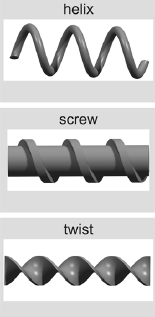
\includegraphics[width=0.4\textwidth]{HelixShapes}
  \caption[Helical microswimmers design]{Three design of helical microswimmers~\citep{peyer2013magnetic}.}
  \label{HelixShapes}
  \end{center}
\end{wrapfigure}
%\end{SCfigure}
%\end{figure}



The artificial smooth flagellum powered by an external magnetic field. 
 The rotating field, i.e. rotational frequency, field strength and angles that 
defined the rotational axis is controlled by the current in the external coil. The helical microrobots rotate 
synchronously with the rotation of the magnetic field and move forward and backward accordingly~\citep{tottori2013artificial}. 
The displacement of the microswimmer along the rotational axis can be measured and the result 
used to calculate the average velocity of the swimmers. There is a linear relationship between an input 
field frequency and swimming speed. According to their result~\citep{tottori2013artificial}, a propulsive force generated by 
the mastigoneme is in opposite direction of the force generated by the main helical filament. 
However, this velocity is only valid if the external force is zero. The proposed 
design~\citep{tottori2013artificial} is rigid and an external stimulus may be used to regulate the swimming
 speed and direction if the swimmer can fold and unfold their structure. 



There are three common shapes of microrobots 
based on the rotary action; a helix, a screw and a twisted ribbon shape around its
 axis (Figure~\ref{HelixShapes}). For the purpose of drilling into solid matter such as biological tissue the screw and helix 
design would be more appropriate. The rotational motion of helical micro
 swimmers is one of the most effective propulsion methods in the low Reynolds number scenarios 
because it leads to translational motion. Microrobots with the microspheres structure perform similarly 
to the helical swimmers and are capable of swimming in the flowing liquid within the microfluidic channel~\citep{kim2013fabrication}. 



There are two main factors that affect the movements of the microrobot in the external magnetic
 field; \hilight{low coercivity and high saturation} magnetization. Also, the motion of the microrobot is related to 
its size given the same magnetic field strength and as such, by increasing the size of the microrobot with the inflexible magnetic material
 volume, the velocity will decrease ~\citep{kim2013fabrication}. 
The surface friction and the drag forces are two resistive forces that impede the microrobot\rq{}s 
motion. Hence, the input magnetic force must be sufficient to overcome these forces for microrobot 
manipulation. Furthermore, the weight of the microrobot requires gravity compensation in the z-direction by 
the magnetic field. The navigation methodology should compensate for gravity to avoid sinking and enable velocity to be 
controlled wirelessly. \citeauthor{mahoney2011velocity} described an algorithm for helical microswimmers velocity 
control plus gravity compensation. In the proposed model the correct pitch angel and 
rotation speed is calculated to achieve the commanded velocity (Figure~\ref{11}).


\begin{figure}
  \centering
    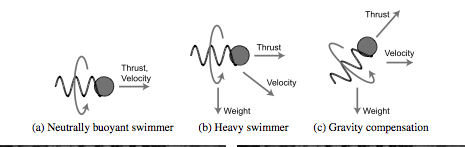
\includegraphics[width=0.9\textwidth]{11}
  \caption[Effect of gravity on swimming microrobot]{The effect of the 
gravity on the microrobot motion direction and gravity compensation~\citep{mahoney2011velocity}.}
  \label{11}
\end{figure}


A magnetic field can be used for controlling teams of microrobots as well as a single 
one. \citeauthor{kim2013fabrication} proposed a method that used a combination of two magnetic materials to 
attain on/off magnetization of each microrobot. The overall control of the group of microrobots 
was achieved by managing the magnetization state of each microrobot. In addition, a second technique has been 
developed for three-dimensional motion of the team of microrobots in a fluidic environment. In
 the latter method, each microrobot is designed in such a way that it uniquely responds to the 
input magnetic field. Therefore, several microrobots can provide feedback position control in 
3D system~\citep{kim2013fabrication}.
An untethered spherical magnetic micromanipulator creates a locally induced rotational fluid flow gradient. 
The created rotational flow propels micro-objects in the flow area. A team of microrobots could perform
 a complex task in micro-transport and micro-assembly~\citep{kim2013fabrication}.

In another study ~\citep{tottori2012magnetic}, a helical microrobot was designed to swim in a low Reynolds number. 
Two designs are selected to run the experiment;  the first one is a bare helical structure and the second one is the
 helical shape with the microholder attached at the end. Both designs will generate the corkscrew
 motion in a fluid environment when the magnetic filed is about few mili Tesla. The second 
design (device with the microholder) is capable of transporting a microobject accurately to the 
target ~\citep{tottori2012magnetic}.


In ~\citeauthor{tottori2012magnetic}\rq{}s study eight designs of microrobots were proposed and tested. 
The uniform static magnetic field was used to explore the magnetic shape anisotropy and the 
magnetic actuation was monitored in the rotating magnetic field. In the static magnetic field the 
set of microrobots had helical angles $\theta$ ranging from ${45^{\circ}}$ to ${70^{\circ}}$ when suspended in the deionised water. 



%\begin{figure}
  %\centering
\begin{wrapfigure}{r}{0.5\textwidth}
  \begin{center}
    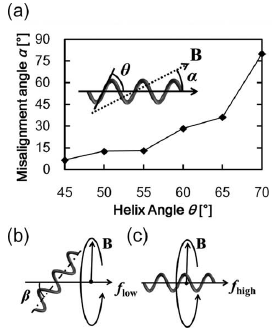
\includegraphics[width=0.5\textwidth]{7}
  \caption[Effect of frequency on microswimmer\rq{}s behaviour]{(a) The misalignment of helical angle $\theta$ with a angle
between megnetic field and helix central axis. (b) the oscillation behaviour
of the microswimmer with the high and low frequencies~\citep{tottori2012magnetic}.}
  \label{ref7}
\end{center}
\end{wrapfigure}
%\end{figure}


This showed (Figure~\ref{ref7}) that a smaller helix angle $\theta$ results in a less misalignment 
angle $\alpha$ because microrobots longest axes will be aligned to the direction of the external magnetic field. 
However in helical microrobot with larger helix angles ($\theta$), the magnetization direction would change to 
the radial axes of the helix  ~\citep{tottori2012magnetic}.
In the rotating magnetic field, the micro helical swimmer exhibits different behaviours depending on 
the strength of the applied frequency in the fixed magnetic field. At low frequencies the micro helix oscillated 
around the helical axes, however the oscillating behaviour changed to the 
corkscrew motion after increasing the applied frequency in the magnetic field. This is similar to characteristics of 
microrobots with an incorporated
 microholder~\citep{tottori2012magnetic}.

The velocity of helical micro swimmers depends on their size and shape. A linear relationship was 
observed between the input frequencies and swimming velocity of the micro swimmers. The outcome of 
the comparison between three microhelixs with the same helix angles showed that the microhelix with the
 greatest diameter has the highest speed, in accordance with the following formula;

\begin{equation}
  U = {\cfrac{(C_n - C_1) \sin \theta \cos \theta}{2(C_n \sin^2 \theta + C_1 \cos^2 \theta)}} \big( d \varpi \big)
\end{equation} 

Where $C_n$ is a drag coefficient perpendicular to the filament and $C_1$ is a drag coefficient
 parallel to the filament. $ \varpi$ is the rotational frequency and $d$ is the rotational diameter of 
the helix ~\citep{tottori2012magnetic}.  



\paragraph{}
The important role of helix angle in the magnetization structure of helical micro swimmers 
was confirmed by \citeauthor{peyer2013bacteria} \citep{peyer2013bacteria}, who used direct laser writing (DLW) as a fabrication method 
 on a \ac*{MPC}. The \ac*{MPC} are non-cytotoxic and showed 
super paramagnetic characteristic because magnetic material was already included in the polymer. 

The relationship between the torque $T$, the drag force $F$, the object\rq{}s velocity $\nu$ and rotational 
speed $\omega$ is linear and modelled by $6\times6$ resistant matrix as below;



\[
\begin{bmatrix} F\\ 
T \end{bmatrix}  =\begin{bmatrix} A & B \\ 
C & D \end{bmatrix}  \begin{bmatrix} \nu
 \\ \omega
\end{bmatrix}
\]




Where $A$, $B$ and $D$ are matrices 3x3 and only depend on the object\rq{}s geometry and fluid velocity.
In the study performed by \citeauthor{purcell1997efficiency} \citep{purcell1997efficiency} has been proved 
matrices $B$ and $C$ are equal ($B = C$) for a typical flagellum. 
There are few methods in use to model the resistance matrices and low Reynolds flow such as the 
method of regularized stokeslets, the boundary element method and the method of fundamental solution
. In designing a microrobot the main parameters required to concentrate on are the helicity angle $\psi$, 
the helix radius $R$, the pitch $p$ and the filament radius $r$ as illustrated in Figure~\ref{ref8} part (c). 

\begin{figure}
  \centering
    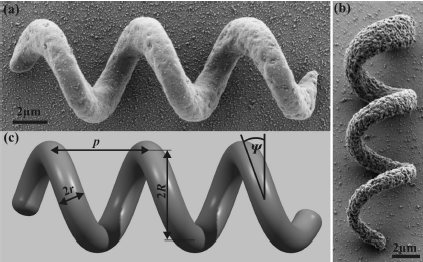
\includegraphics[width=0.7\textwidth]{8}
  \caption[The prototype of microhelical device]{ The prototype of microhelical device. (a) Scanning electron microscopic image of the micro polymer composite
with the 2 vol.\% nanoparticle fill factor and (b) 4 vol.\% of nanoparticle fill factor. (c) The CAD model
shows all the parameters required for the microhelical design ~\citep{peyer2013bacteria}.}
  \label{ref8}
\end{figure}






%\begin{figure}
%  \centering
\begin{wrapfigure}{r}{0.5\textwidth}
  \begin{center}
    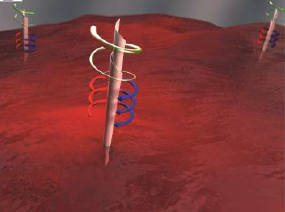
\includegraphics[width=0.5\textwidth]{nanoJet3}
  \caption[Drilling motion of a nanotube]{Demonstrating the drilling motion of the nanotubes under rotating
 magnetic field~\citep{C2NR32798H}.}
  \label{nanotube}
\end{center}
\end{wrapfigure}
%\end{figure}



Magnetic actuated microrobot is divided into two categories; torque driven microrobot and force
 driven microrobots.
The micro robot using the torque-driven method is more favourable than the force-driven method 
because their rotation is based on applying torque rather than a force to pull the device ~\citep{peyer2013bacteria}.



Another approach for powering a micro robot is using the catalytic conversion of chemical energy
 into mechanical energy (Figure~\ref{nanotube}). In this method, the catalyst accelerates the consumption of hydrogen peroxide
 and helps the self-propulsion of micro robot to pump the fluid to transport cells and colloidal 
particles ~\citep{C2NR32798H}. The catalytic tube is fabricated with a sub micrometer diameter.
 This technique is not applicable for the minimally invasive surgery (MIS) yet because the catalytic
 material used in the fabrication process of nanotubes is toxic. Hence, biocompatible fuel is required to be developed in order to 
apply this technique in a live cell environment~\citep{C2NR32798H}.




Alternatively, the micro driller can be powered and controlled by using an external magnetic field 
such that changes in the frequency of the rotating magnetic field switch the rotational orientation of the 
micro tool from the horizontal position to the vertical one. The vertical orientation of the rolled up microtube 
and its sharp helical design makes the device suitable for drilling into biological tissue. In addition, the micro 
driller can be used for targeted drug delivery in MIS ~\citep{C2NR32798H}. 


\subsubsection{Plant-based microrobots}
%\hilight{details about fabrication, extract xylem tissue}
The helical microstructures are not limited to having flagellum-like structures and microbots with
general cilia-like feature have been designed. \citeauthor{gao2013bioinspired}
 observed the helical microstructures that imitates spiral water-conducting vessels of different plants. 

\begin{figure}
  \centering
    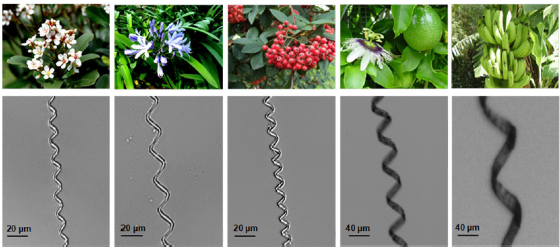
\includegraphics[width=0.9\textwidth]{plants}
  \caption[Xylem\rq{}s shape in different plants ]{The shape of the Xylem in differnt plants~\citep{mahoney2011velocity}.}
  \label{plants}
\end{figure}

In order to obtain unstretched spiral vessel several plants were collected and their leaves were 
macerated and washed with pure water. Tweezers were used to uncover compressed spiral vessels 
in the planar networks. Leaves were gently scored and two segments were pulled apart to a permanent
 length to stretch the spiral vessels. These spiral vessel were kept in a glass slides and covered with a 
thin layer ($20 nm$) of titanium and nickel ($80 nm$) using an 
E-beam evaporator ~\citep{mahoney2011velocity}. The helical vessels were coated in nail 
polish and baked for 2 minutes to impound the helix and protect the structure. The final product is 
a photoresist film on glass that was cut into required lengths.      
  

The fabrication process involves coating isolated spiral xylem vessel plant fibres within a (Figure~\ref{ref8})
thin magnetic layer. Xylem tissue transports the plant\rq{}s required food such as water and other 
nutrition from the root to the leaves using capillary action ~\citep{mahoney2011velocity}.
Use of plant material in this method enables simple three-dimensional microswimmers fabrication 
and biocompatibility. In addition, the magnetic cover helps to ensure accurate directional control and 
high-speed propulsion. Therefore the fabrication processes were extremely simplified as the main 
component of the helical microswimmers is from nature and more than a million individual micro helicals 
can be made from a very small section of the plant stalk ~\citep{mahoney2011velocity}. Using mechanical stretching can control geometric variables of the helical vessels such as the pitch and
 helix angle and hence plenty of helical microswimmers can be reproduced. The final shape of the 
helical microswimmer is determined mainly by the initial diameter of the unstretched spiral vessel. The
 process of stretching helical plant structure was performed via plastic deformation so that the number 
of helical turns are constant and tensile stretching of the plant fibre stretching is negligible~\citep{mahoney2011velocity}. 


%\begin{figure}
%  \centering
\begin{wrapfigure}{r}{0.5\textwidth}
  \begin{center}
    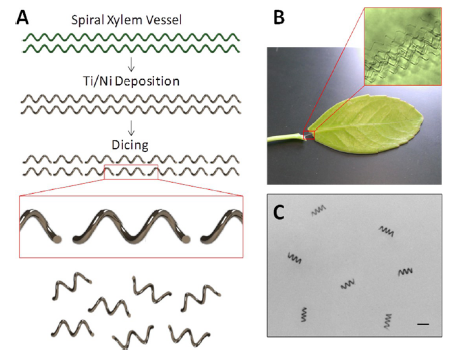
\includegraphics[width=0.5\textwidth]{plants2}
  \caption[plant-based microrobot]{(A) The stages were required to make a plant-based microrobot. (B) A microscopic image of the 
a xylem helical structure~\citep{gao2013bioinspired}.}
  \label{plants2}
\end{center}
\end{wrapfigure}
%\end{figure}


The method used for precise propulsion control and characterising the locomotion behaviour of the 
plant-based microswimmers is similar to the method applied in \citeauthor{gao2013bioinspired} study.

According to \citeauthor{gao2013bioinspired} ~\citep{gao2013bioinspired} experiment, the plant-based 
microswimmers exhibited high speed movement ($85~\mu m$) in raw biological medium such as 
pure human serum under the rotating magnetic field. However, their swimming speed in pure water
 ($90~\mu m$) was slightly higher than human serum.   
 Hence, an increased velocity of the 
biological fluid has a minor effect on the plant-driven microswimmers, which is an important 
advantage of this microdevice over the common microrobots%\hilight{WHY}.



\subsection{Actuation methods} \label{actuation}

The actuation method for swimming microrobot should meet two main criteria in order to be 
applicable. The method needs to be appropriate in the fluid environment and can be applied 
in the micro scale. One approach was using tethered and onboard motor to an external power
 source to actuate the microrswimmers, but this approach will not be realistic in micro scale. 
Therefore, using the propulsion mechanism of natural swimmers such as flagellum demonstrated 
a successful result~\citep{peyer2013bio}.

Another approach is using electrochemical decomposition for microrobot locomotion. 
The mechanism of these types of artificial microdevice is similar to bacteria as both harvesting the 
required energy from their environment. In that case, the environment contains chemical material such 
as hydrogen peroxide to make the electrochemical reaction. The successful application of these catalyst 
microdevice in vitro is reported for cell transportation. However, this approach will not be suitable for in vivo 
cases which chemical material may harm human body~\citep{peyer2013bio}.   

Therefore, the idea of using magnetic field for the microrobot actuation was satisfied both requirements. 
Applying the low strength magnetic field is harmless for human body and that can be used within fluidic 
environment. So we can have microswimmers in the fluid environment and control them remotely. But, 
there are still challenges with using magnetic field as an actuation method. The magnetic field will decay 
fast by increasing the distance from the magnetic source. Thus, that factor needed to be considered 
when preparing the set up for actuated microrobot~\citep{peyer2013bio}.   

The microrobot actuation by magnetic field can be force driven or torque driven. In case of the torque 
driven, the magnetized microrobot experiences a torque that perform to align its magnetization with the 
external magnetic field. The magnetic torque and force are formulated as follow;



\begin{equation}
  \bm{T}_m = V\bm{M} \times \bm{B}
\label{originalForce}
\end{equation}


\begin{equation}
  \bm{F}_m = V(\bm{M\nabla}) \bm{B}
\label{originalTorque}
\end{equation}

Where $\bm{T}_m [N.m]$ is torque, $\bm{F}_m [N]$ is force, $\bm{M} [A.m^{-1}]$ is magnetization, $V [m^3]$ is
volume of a magnetized object and $\bm{B} [T]$ is the magnetic field. If we have a hard magnet, $\bm{M}$ becomes
a constant or it can be a function of the geometry of the object and applied field. In the uniform magnetic field, 
there is no force and microrobot just experiences the torque until the magnetization $\bm{M}$ is collinear with the
magnetic field. At this point, there is no torque and microswimmer stays stationary. Thus, a magnetic field is required 
to go through spatial or temporal changes to generate a continous actuation. This can be performed by 
rotating the helmholtz coils or generaring dynamic magnetic fild by using AC current~\citep{peyer2013bio}.




\subsection{Fabrication methods} \label{fabrication}

Historically, the fabrication of the microrobot was the main problem that recent fabrication methods 
offer a feasible solution~\citep{gao2013bioinspired}.
In 2007, the first artificial bacteria flagella was fabricated based on thin-film deposition and self-scrolling
 methods~\citep{qiu2014noncytotoxic}.\hilight{In this method}. They used InGaAs/GaAs bilayer for fabricating
helical tail and Ni for actuation microrobot\rq{}s head. The similar fabrication method employed by Zhang
 in 2009 with the addition of a Cr layer between the microrobots\rq{} tail and its head~\citep{qiu2014noncytotoxic}.
An improved adhesion of microrobot was the result of adding Cr layer. 

3D laser direct writing (DLW) and electron beam decomposition are methods used since then. A typical 
fabrication process consists of two stages. Initially the core structure of the artificial helical 
microswimmer is printed using 3D lithography and then electron beam evaporation is used for 
ferromagnetic thin film coating~\citep{tottori2013artificial}.  
Performance of each microswimmer (with different design) can be imaged by the scanning electron
 microscope (SEM). After the fabrication process is completed, the next step is to release the structure into 
deionised water using the tungsten probe. The tank with deionised water is installed in the middle of the 
three-axis Helmholtz setup. 




\begin{figure}
  \centering
%\begin{wrapfigure}{r}{0.5\textwidth}
 % \begin{center}
    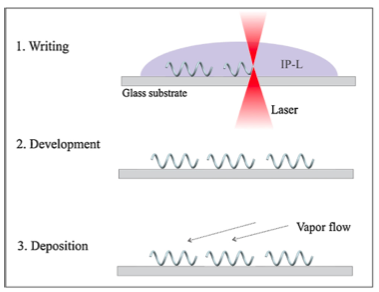
\includegraphics[width=0.7\textwidth]{tempreture}
  \caption[Direct lasor writing]{DLW steps. step 1 is writting helical microrobots, in step 2 microrobots were 
developed in isopropyl alcohol and step 3 is coating them by a layer of Ni and Ti. ~\citep{qiu2014artificial}.}
  \label{tempreture}
%\end{center}
%\end{wrapfigure}
\end{figure}




To improve biocompatibility for in-vivo applications, the 
microrobot can be covered with a thin layer of titanium. In addition, the microrobot\rq{}s structure was layered with 
nickel for the purpose of magnetic actuation.

\citeauthor{qiu2014artificial}~\citep{qiu2014artificial} reported a successful application of helical microrobots
for drug delivery were known as \lq\lq{}smart\rq\rq{} drug carriers. Again, they used DLW for the fabrication method 
as shown in the Figure \ref{tempreture}. 



The smart drug carriers were coated in a layer of temperature-sensitive liposomes which is composed 
of a lipid bilayer and was proposed for cancer therapy in local hyperthermia treatments~\citep{qiu2014artificial}.
The main component of temperature-sensitive liposomes is Dipalmi- toylphosphatidylcholine (DPPC) which
transforms from solid to liquid gel at the $41^{\circ} C$ and released encapsulated drugs.

\paragraph{}
 \citeauthor{qiu2014noncytotoxic}~\citep{qiu2014noncytotoxic} were used commercially available material such as ORMOCOMP
 for fabrication of helical microrobots in their recent experiment. ORMOCOMP is a biocompatible photoresist which
can improve the potential use of microrobots for in vivo applications becuase it supports viability, cell proliferation
 and normal morphology of various cell lines. For the purpose of magnetic microrobot actuation, soft magnetic material
such as Fe, Ni and Co are commonly used in microscale structures. The main reason is their biocompatibility
with surface decomposition methods, however Ni and Co are cytotoxic and pure iron can be biodegradable~\citep{qiu2014noncytotoxic}.
ORMOCOMP helical swimmers were coated onto a thin layer of Fe ($25 nm$) using electron beam decomposition.
  




\begin{comment}

The review of all the fabrication methods used for the micrordevice is represented in the table\ref{fabrication_table}.

\begin{table}[!ht]

\centering% used for centering table
{\rowcolors{2}{gray!100!brown!70}{gray!50!yellow!30}
\begin{tabular}{c c c c c c c c}% centered columns (8 columns)
\toprule[2.0pt]



\head{Author} & \head{Shape} & \head{Length} & \head{Pitch} & \head{Pitch-angle} & \head{Radius} & \head{Filament-radius} & \head{Speed}\\

%heading
\midrule
%\hline% inserts single horizontal line
Arcene 	& 	    		  & 	1000		& 	1000		& 	1000		& 	1000		& 	1000		& 	1000\\% inserting body of the table
Dexter 	& 	Sparse 		  & 	20000	& 	1000		& 	1000		& 	1000		& 	1000		& 	1000\\
Dorothea & 	Sparse 		  & 	10000	& 	1000		& 	1000		& 	1000		& 	1000		& 	1000\\[1ex]% [1ex] adds vertical space



\bottomrule[2.0pt]
\end{tabular}
}
\label{fabrication_table}% is used to refer this table in the text
\caption{Microrobot\rq{}s fabrication methods}\label{fabrication table}% title of Table
\end{table}

\end{comment}

%%%%%%%%%%%%%%% Table %%%%%%%%%%%%%%
\begin{table}[h!]
  \centering

\setlength{\arrayrulewidth}{.6mm}
\setlength{\tabcolsep}{1pt}
\renewcommand{\arraystretch}{2.8}


  \begin{tabular}{ c m{2.5cm}  m{4.3cm} m{3cm} m{2cm}}
    \hline
\rowcolor{lightgray}
    Microrobot Image & Design  & Fabrication Method & propulsion method	&Citation  \\ \hline\hline



    \begin{minipage}{.3\textwidth}
      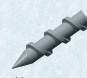
\includegraphics[width=\linewidth, height=25mm]{screw_ta}
    \end{minipage} 
    &
    \begin{minipage}[t]{3cm}
      \begin{itemize}
        \item Helical Screw Shape
    
      \end{itemize}
    \end{minipage}
    & 
    \begin{minipage}{4cm}
      \begin{itemize}
        \item Direct Laser Writting (DLW)
	\item Two-photon Polymerization
   
      \end{itemize}
    \end{minipage}
	&

  \begin{minipage}[t]{3cm}
      \begin{itemize}
        \item RFT
    
      \end{itemize}
    \end{minipage}
	&
	 \begin{minipage}[t]{3cm}
	   \begin{itemize}
        \item \citep{peyer2013magnetic}
   
      \end{itemize}
	 \end{minipage}
    \\ \hline
%%%%%%%%%% Second Row

 \begin{minipage}{.3\textwidth}
      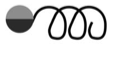
\includegraphics[width=\linewidth, height=25mm]{helical_rigid_tail}
    \end{minipage}
    &
    \begin{minipage}[t]{3cm}
      \begin{itemize}
        \item Helical rigid tail
      
      \end{itemize}
    \end{minipage}
    & 
    \begin{minipage}[t]{4cm}
      \begin{itemize}

        \item Direct Laser Writting (DLW)
	\item Two-photon Polymerization
   
      \end{itemize}
    \end{minipage}

	&
  \begin{minipage}[t]{3cm}
      \begin{itemize}
        \item RFT
    
      \end{itemize}
    \end{minipage}

	&

	   \begin{itemize}
        \item \citep{peyer2013bio}
   
      \end{itemize}
	
    \\ \hline

%%%%%%%%%%%%%%%% Third row

\begin{minipage}{.3\textwidth}
      \includegraphics[width=\linewidth, height=25mm]{Planar_flexible_tail}
    \end{minipage}
    &
    \begin{minipage}[t]{3cm}
      \begin{itemize}
        \item Planar flexible tail
     
      \end{itemize}
    \end{minipage}
    & 
    \begin{minipage}[t]{4cm}
      \begin{itemize}
        \item The EMA coil system
     
      \end{itemize}
    \end{minipage}
 &
  \begin{minipage}[t]{3cm}
      \begin{itemize}
        \item SBT
	\item RFT
     
      \end{itemize}
    \end{minipage}

	&
	   \begin{itemize}
        \item \citep{kim2013fabrication}
   
      \end{itemize}
    \\ \hline

%%%%%%%%%%%%% Forth row

\begin{minipage}{.3\textwidth}
      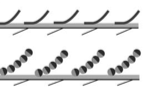
\includegraphics[width=\linewidth, height=25mm]{cilia-shape}
    \end{minipage}
    &
    \begin{minipage}[t]{3cm}
      \begin{itemize}
        \item Cilia
     
      \end{itemize}
    \end{minipage}
    & 
    \begin{minipage}[t]{3cm}
      \begin{itemize}
        \item The EMA coil system
     
      \end{itemize}
    \end{minipage}
&
  \begin{minipage}[t]{4cm}
      \begin{itemize}
        \item SBT
	
     
      \end{itemize}
    \end{minipage}

&
	 \begin{minipage}[t]{3cm}
	   \begin{itemize}
        \item \citep{kim2013fabrication}
   
      \end{itemize}
   \end{minipage}
    \\ \hline



%%%%%%%%% Fifth Row
 \begin{minipage}{.3\textwidth}
      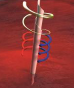
\includegraphics[width=\linewidth, height=25mm]{tube_ta}
    \end{minipage}
    &
    \begin{minipage}[t]{3cm}
      \begin{itemize}
        \item Nanotube
        
      \end{itemize}
    \end{minipage}
    & 
    \begin{minipage}{4cm}
      \begin{itemize}
        \item Molecular Beam Epitaxy (MBE)
	   
	   
    
      \end{itemize}
    \end{minipage}
	&




	&
	   \begin{itemize}
        \item \citep{C2NR32798H}
   
      \end{itemize}
    \\ \hline

%%%%% Sixth Row

 \begin{minipage}{.3\textwidth}
      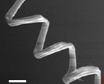
\includegraphics[width=\linewidth, height=25mm]{plant_ta}
    \end{minipage}
    &
    \begin{minipage}[t]{3cm}
      \begin{itemize}
        \item Plant-based
      
      \end{itemize}
    \end{minipage}
    & 
    \begin{minipage}[t]{4cm}
      \begin{itemize}
        \item Macerating Plant\rq{}s Leaves
	\item Seperating Spiral Vessels
	\item Stretching spiral Vessels
	\item Coating with Ti

      \end{itemize}
    \end{minipage}
	&



	&
	   \begin{itemize}
        \item \citep{gao2013bioinspired}
   
      \end{itemize}
    \\ \hline

%%%%%% Seven Row

 \begin{minipage}{.3\textwidth}
      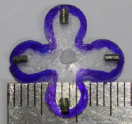
\includegraphics[width=\linewidth, height=25mm]{Jelly}
    \end{minipage}
    &
    \begin{minipage}[t]{3cm}
      \begin{itemize}
        \item Jellyfish
     
      \end{itemize}
    \end{minipage}
    & 
    \begin{minipage}[t]{4cm}
      \begin{itemize}
        \item The EMA coil system
     
      \end{itemize}
    \end{minipage}
&



	&
	   \begin{itemize}
        \item \citep{ko2012jellyfish}
   
      \end{itemize}
    \\ \hline








  \end{tabular}
  
  \caption[Summery of microrobots\rq{}s desing, locomotion and fabrication]{Different types 
of microrobots and their fabrication method.}\label{Micro}
\end{table}


%%%%%%%%%
%%%%%%%%%%%%%%%%%%%% Method %%%%%%%%%%%%%
%%%%%%%%%

\chapter{Methods}

In this chapter the design of microhelix is described and a few number of design is presented. It followed by introducing
the fabrication mechanism, the technology applied to fabricate microstructures and post-processing fabricated microstructres.
The simulation is major part of this chapter which is modelling the swimming mechanism of microhelix in high viscous fluid. 
Three models studied for describing the swimming motion of the microhelix and one model (\ac*{RFT}) is implemented to simulate
microhelix with two and six degree of freedom. The torque driven magnetic field is selected to actuate the microhelix and
as a result the relation between the rotational velocity and translational velocity is achieved.    







%%%%%%%%%%%%%%%%%%% Design %%%%%%%%%%%%%%%
\section{Microrobot design} \label{microDesign}

For the purpose of this study, the design of microrobots is focuced on a helical 
tail shape with possible propeller head. The helical shape microrobot is generally copied the design of the helical 
rigid tail flagellum which is one-dimensional structure. There are other microstructures 
such as cilia and planar flexible tail flagellum that are copied to build a swimming microrobot. The 
helical rigid tail flagellum is a preferred design for the micro swimmer as its simplicity makes
 it feasible to copy in micro scale. In addition, its swimming mechanism is more efficient than 
other type of microswimmers \citep{peyer2013bio}. 
Therefore, the key characters of the helix were 
identified and all the design was based on optimising these characters. 


 
\begin{figure}
        \centering

  \begin{subfigure}[b]{0.25\textwidth}
                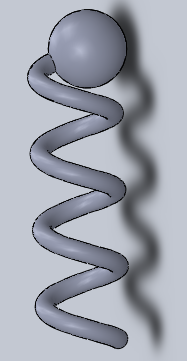
\includegraphics[width=\textwidth]{Design6}
                \caption{Circle base helix with sphere head}
                \label{Design6}
        \end{subfigure}~
  \begin{subfigure}[b]{0.36\textwidth}
                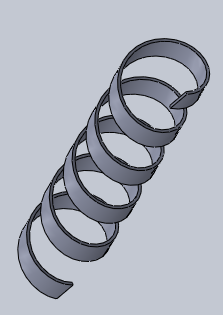
\includegraphics[width=\textwidth]{Design2}
                \caption{Rectangle base helix}
                \label{Design2}
        \end{subfigure}~
  \begin{subfigure}[b]{0.32\textwidth}
                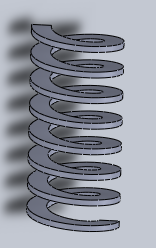
\includegraphics[width=\textwidth]{Design3}
                \caption{Rectangle base helix}
                \label{Design3}
        \end{subfigure}
        \begin{subfigure}[b]{0.335\textwidth}
                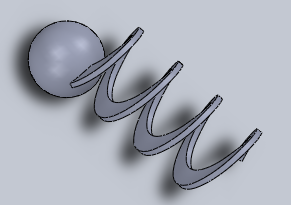
\includegraphics[width=\textwidth]{Design4}
                \caption{Rectangle base helix with sphere head}
                \label{Design4}
        \end{subfigure}~
  \begin{subfigure}[b]{0.37\textwidth}
                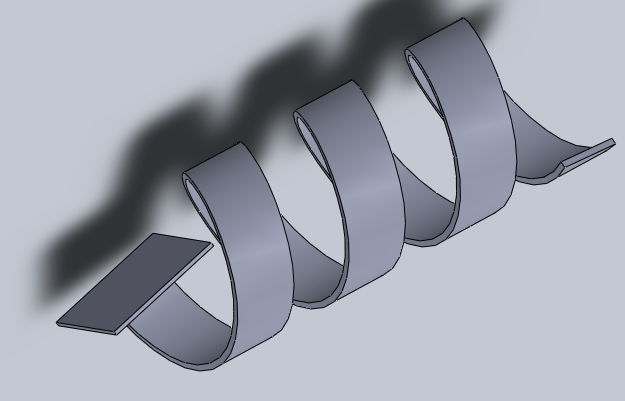
\includegraphics[width=\textwidth]{Design5}
                \caption{Rectangle base helix with square head }
                \label{Design5}
        \end{subfigure}~
  \begin{subfigure}[b]{0.222\textwidth}
                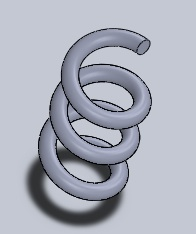
\includegraphics[width=\textwidth]{Design1}
                \caption{Circle base helix}
                \label{Design1}
        \end{subfigure}
      
        \caption[Different helical designs]{}\label{Different helical designs}

   %add desired spacing between images, e. g. ~, \quad, \qquad, \hfill etc.
          %(or a blank line to force the subfigure onto a new line)
       
         %add desired spacing between images, e. g. ~, \quad, \qquad, \hfill etc.
          %(or a blank line to force the subfigure onto a new line)

\end{figure}

The figure \ref{Different helical designs} represents the
variaty of designs have been tried in the design stage of this project. A circle base helix with (\ref{Design6}) 
and without sphere head (\ref{Design1}) has been tried. Also their pitch, helical angle and length of the helix
were changed to monotor its behaviour druing simulation and fabrication process. Two types of
 rectangle base helix has designed. In the first one, the larger side of the rectangle revolves around a spiral path (\ref{Design2})
whilst in the second one the smaller side of the rectangle revolves around the spiral path (\ref{Design3}).
The former design advantages in the simulation process because its shape produce larger force to propell the microrswimmer.
However, the it behave poorly in the fabrication process becase it has not provide sufficient suface area to contact with the 
substrate. Therefore we can\rq{}t print it vertically. The latter provides strong base for printing vertically but ca\rq{}t generate 
sufficient force to move the microswimmer forward. The new design of microhelix which has
variable pitchrather than constant pitch is made (\ref{Design7}) and fabricated vertically. The advantage of variable pitch design 
is providing strong base to fabricate it vertically. 

%\begin{figure}
%  \centering
\begin{wrapfigure}{r}{0.55\textwidth}
  \begin{center}
    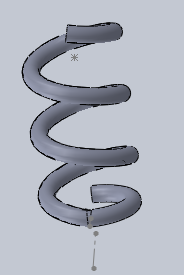
\includegraphics[width=0.4\textwidth]{Design7}
  \caption[Variable pitch helix design]{Variable pitch helix design}
  \label{Variable pitch helix design}
\end{center}
\end{wrapfigure}
%\end{figure}





%%%%%%%%%%%%%%%%%% Fabrication %%%%%%%%%%%%%
\section{Microrobot fabrication} \label{microFabric}

The main challenge of the fabrication process is not just fabricating the extremely small object. 
There are number of other factors that need to be considered to select an appropriate approach for 
fabricating helical shape mincrorobot. An ideal fabrication approach should have control over design 
parameters and in particular it should be suitable for applying magnetic material
 for the actuation purpose \citep{peyer2013bio}.

The complete fabrication process is summarised in the diagram \ref{Fabrication diagram}.
The process started by importing the structure files into the software called Describe for 
the pre-processing purpose. The structures file contains all the microrobots that is designed by the 
software called Solidwork. The next stage is writing the structure using nanoscribe facility, which is 
done in the clean room. After few hours, the structures will be ready and they can be seen under 
the \ac*{SEM}. However, the structure made of polymer and the pictures of non-metal object under 
the \ac*{SEM} is not perfect. Thus the polymer made microrobot were coated with the layer of 
metal (usually gold) first, this process called sputtering coating process.  At this stage, the 
picture of microrobot were analysed under the \ac*{SEM} and if they are satisfactory, they will go t
o the final stage which is magnetization process. However, we never try the magnetization stage 
in this project because the aim was to optimise the structures in terms of design and fabrication and 
there was no plan to run an experiment within the short period of time. The pictures were encountered 
to have a problem were sent to the design stage for further optimisation process. In the following 
two sections, we will explain the mechanism of the two photon lithography technique and \ac*{SEM} in
 more details.   




%%%%%%%%%%%% Overview Diagram of the fabrication process %%%%%%%%%%%%% 

\begin{figure}
\centering
\begin{tikzpicture}[scale=1.10,transform shape]

  % Draw diagram elements
  \path \Step{1}{Preparing};
  \path (p1.south)+(0.0,-1.5) \Step{2}{Production};

  \path (p2.south)+(0.0,-1.5) \Step{3}{Post-processing};
  \path (p3.east)+(3.0,0.0) \Step{4}{Sputter Coating};
  \path (p4.south)+(0.0,-1.50) \Step{5}{Image Ananlysis};

 \path (p5.east)+(3.0,0.0) \Step{6}{Coating Magnetic Material};
  %\path (p4.east)+(5.0,0.0) \practica{7}{Calculate forward and inverse kinematic};
  %\path (p5.east)+(5.0,0.0) \practica{8}{Design feedback control mechanics};

  %\path (p5.south)+(3.5,-2.0) \practica{9}{Integrating e-AR and robot};
  %\path (p9.south)+(0.0,-1.5) \practica{10}{Laparoscopy Robot};


  % Draw arrows between elements
  \path [line] (p1.south) -- node [above] {} (p2);
  \path [line] (p2.south) -- node [above] {} (p3);
  \path [line] (p3.east) -- node [above] {} (p4);
  \path [line] (p4.south) -- node [above] {} (p5);

 \path [line] (p5.east) -- node [above] {} (p6);
%  \path [line] (p7.south) -- node [above] {} (p8);

  %\path [line] (p5.south) -- node [above] {} (p9);
  %\path [line] (p8.south) -- node [above] {} (p9);
 % \path [line] (p9.south) -- node [above] {} (p10);



  \background{p1}{p1}{p3}{p3}{Nanoscribe }
  \background{p4}{p4}{p5}{p5}{SEM}
  

 % \path [line] (p5.south) -- node [above] {} (bk3-n);
 % \path [line] (bk3-s) -- node [above] {} (p8);
 % \path [line] (bk3-s) -- node [above] {} (p9);
  %\path (bk1-e)+(+6.0,0) node (ur1)[ur] {};
 % \path (bk2-w)+(+6.0,0) node (ur2)[ur] {};
  %\path (bk3-w)+(+3.0,0) node (ur3)[ur] {};
% \transreceptor{bk1-e}{pre processing}{ur1};
 % \transreceptor{bk2-w}{Feature selection}{ur2};
  %\transreceptor{bk3-w}{classification}{ur3};


%%%%%%%%%%%%%% CHANGED%%%%%%%%%%%%%
\end{tikzpicture}									   %
\caption[Fabrication overview]{Fabrication diagram. The nanoscribe technology is employed
for the fabrication process and it followed by analysing structure under SEM. 
The final stage (yellow block in third column) has not been tried in this project. }						   %
\label{Fabrication diagram}										   %
\end{figure}										   %	
												   %
%%%%%%%%%%%%%% CHANGED%%%%%%%%%%%%%




%%%%%%%%%%%%%%%%%%%%%%%%%%%%%%%%%%%%%%%%%%%%%%%%

\subsection{Nanoscribe}\label{nanoscribe}

Nanoscribe is the company provide sophisticated system and device for true 3D
 micro and nanofabrication. Their system is based on the laser lithography and it 
used two-photo polymerization technique for the fabrication. The fabrication device combines 
two modes for writing; the high-speed galvo-mode and an ultra-precise piezo-mode. The former 
is for fastest fabrication and it makes the structure in a layer-by-layer process. The latter is mainly for
 printing arbitrary 3D trajectories~\citep{Doe:2014Feb:Online}. The complete nanoscribe 
package made of three components, Photonic Professional GT, the software and IP Photoresists. 
Photosensitive material is used in both modes for structuring arbitrary 3D patterns in a high-resolution. 
The properties of the photosensitive material, the laser power and the size of the spot in the material are
 determined the voxel size. Extremely small voxel size can be achieved when focusing optics is used with 
a high numerical aperture. The fabrication process in each mode is based on moving the voxel relative to
 the sample. The galvo mode approach is called \ac*{MBFS} which the laser beam is scanned 
galvanometric mirrors and piezo-actuators will control the vertical movement. However in 
piezo-mode, piezo actuators is moving the substrate in all three dimensions to achieve highly 
precise focus trajectory. This type of implementation is know as \ac*{FBMS}~\citep{Doe:2014Feb:Online}.




\begin{figure}
  \centering
    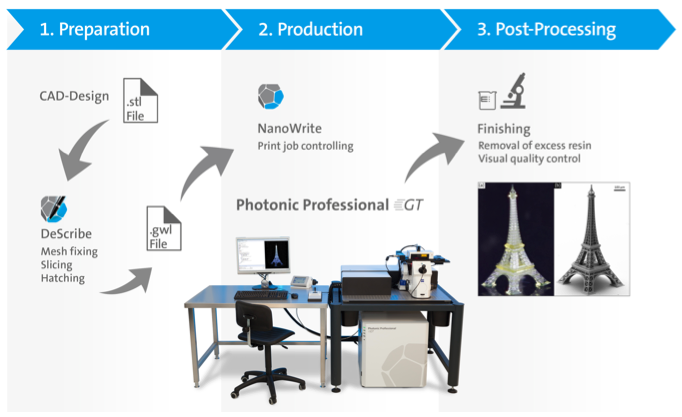
\includegraphics[width=0.9\textwidth]{nanoscribeWorkflow}
  \caption[Nanoscribe workflow]{nanoscribe workflow. The stages are inveolved in  3D micro-printing with nanoscribe
 device is shown in the diagram~\citep{Doe:2014Feb:Online}.}
  \label{nanoscribeWorkflow}
\end{figure}



\paragraph{}
The whole process of fabrication is formed of three stages; preparation, production and post-processing. 
In the first stage, the \ac*{stl} file that contains the design of structures will import into the software tool
 called DeScribe. In this software, each design will go though three steps for fixing the mesh, slicing and
 hatching. By completing these three steps, the result will be the \ac*{gwl} format file that is ready for the 
production stage.   
The production is the stage for controlling the print job that has been done by user-friendly
 graphical interface software, NanoWrite. This software controls different aspect of the lithography 
system such as autofocus, exposure dose and substrate positioning.  
The final stage is removing the excess resin to improving the visual quality~\citep{Doe:2014Feb:Online}. 

IP Photoresists is a high viscose fluid that comes as part of nanoscribe package. It is
 used to maximise the performance of the multiphoton polymerization process. It has high 
mechanical stability and stick to different substrate very well~\citep{Doe:2014Feb:Online}. A wide
 range of material with different mechanical, optical or chemical properties can be used for the substrate 
in direct laser writing. The choice of the substrate material is an application dependent. For example in 
optical applications the transparent material such as glass is more appropriate. In the latter application 
substrate is mainly for supporting to the polymer structures. Also, we can use pre-structured substrates 
such as transparent micro-fluidic chip that polymer structure can be printed on the substrate. In that
 case, the functionality of multiphoton lithography can be improved by combining the mechanical parts 
with substarte~\citep{Doe:2014Feb:Online}.  

\paragraph{}
In this project we used nanoscribe device to print microswimmers using the galvo-mode of the machine. 
The whole printing unit is located in the clean room\footnote{Clean room is an environment with controlled
  concentration of airborne particle to make it suitable for product manufacturing~\citep{Doe:2014April:Online}. }. 
The fabricated structures were observed under the 
\ac*{SEM} and all the images result will be presented and discussed in the result \ref{result} and discussion
chapters \ref{discussion} respectively.


\subsection{Scanning Electron Microscope (\ac*{SEM})}\label{sem}



%\begin{figure}
%  \centering
\begin{wrapfigure}{r}{0.5\textwidth}
  \begin{center}
    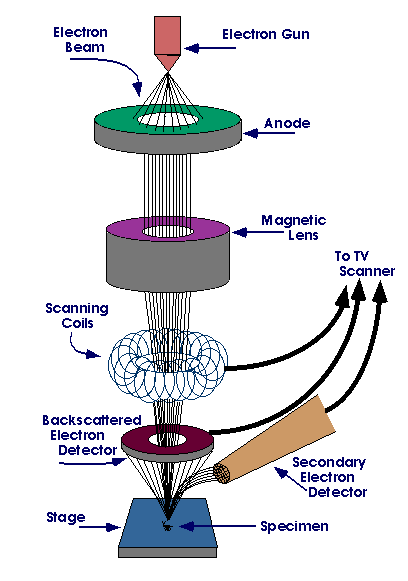
\includegraphics[width=0.5\textwidth]{SEM}
  \caption[Scanning Electron Microscope]{Scanning Electron Microscop. The components of the \ac*{SEM} is shown 
in the diagram~\citep{Doe:2014Jan:Online}.}
  \label{SEM}
\end{center}
\end{wrapfigure}
%\end{figure}


\ac*{SEM} is a powerful device for obtaining high magnification images to analyse and examine
 the material or individual features. \ac*{SEM} is invented 50 years ago and it is used extensively 
in diverse scientific fields such as biology, medicine or metallurgy,  to name just a few. The \ac*{SEM} can 
provide images with the high-resolution dawn to $25$ Angstroms.\footnote{$1 ~\ Angstrom =
1.0 \times 10^{-10} Metres$}%~\citep{Doe:2013Dec:Online}.



\ac*{SEM} generates a range of signals at the surface of solid specimens by using a focused beam
 of high-energy electrons. The process is started from producing electron beam by the electron gun 
at the top of the microscope and then travels into the microscope. The microscope is placed in the
 vacuum. Then the beam focused down into the specimen by passing through the electromagnetic
 fields and lenses. Once the focused electron beam interacts with the specimen, electrons are revealed 
from the specimen. At this point, the back-scattered electrons are collected by the detectors and were 
converted into variety of signals. Ultimately, generated signals sent to the screen to form the final image 
of the specimen\citep{Doe:2014Jan:Online}. 



The key advantages of using \ac*{SEM} over traditional microscope is having a large depth of
 field and also higher resolution. In addition, researchers has more control over the degree of 
magnification because \ac*{SEM} uses electromagnets\citep{Doe:2014Jan:Online}.

We need to prepared samples before using the \ac{SEM} because it using the electron in the
 vacuum condition. That means sample should not contain any water otherwise the water will 
vaporise in the vacuum. This is high-vacuum \ac*{SEM}. If we require an image of a wet sample such 
as biological specimen we can use the low-vacuum \ac*{SEM}. In that case, the specimen chamber
 contains air that avoid dehydrating of samples.
Because the produced images are based on the electron-sample interaction, if the sample is made
 of non-metal material, the final image is not very clear. Thus, they need to be covered by a metal to
 make it conductive. The process of covering the sample with metal is called sputter coating\citep{Doe:2014Jan:Online}.

\paragraph{sputter coating}
In the sputter coater, there is small chamber in the vacuum to place the sample in. An electric field 
and argon gas used in order to release the electron from the argon and convert it into positive charged 
atom. Then, argon ions and negatively charged gold foil are attracted to each other and as a result gold 
atoms fall from the surface of the gold and settle onto the surface of the specimen. Therefore a thin gold 
layer covers the surface of the sample and make it conductive for \ac*{SEM} machine\citep{Doe:2014Jan:Online}.

In this project, the microrobot structure is made of polymer and we made them conductive by applying the 
sputter coating process and then analysed them under \ac*{SEM}. The images of the microrobot structures 
before and after coating is presented in the result section \ref{result}. In the following section, the simulation of 
microrbot is demonestareted in detail.



%%%%%%%%%%%%%%%%%% Simulation %%%%%%%%%%%%%
\section{Simulation}\label{simulation}
The simulation of the microrobot is formed by two main components; helical microrobot propulsion mechanism
 and actuation method. The complete algorithm that describes the implementation of the simulation
system is represented in the diagram \ref{Simulation algorithm}. In this algorithm, the desired velocity is given to the system
and the required electric current to make the dynamic magnetic field will be an output. The pseudocode of
the algorithm \ref{PSuedocode} is provided more details in each step of the implementation and the complete computation
is explained in section \ref{RFT_sixDegree} and section \ref{microActuation}.    


\begin{comment}

\begin{figure}
\centering
\begin{tikzpicture}[scale=1.30,[every node/.style={font=\large,
  minimum height=1.5cm,minimum width=0.8cm},]]

  % Draw diagram elements
  \path \Step{1}{Desired Velocity};
  \path (p1.east)+(3.0,0.0) \Step{2}{Propulsion Algorithm};
 \path (p2.east)+(3.0,0.0) \Step{3}{Actuation Algorithm};
   \path (p3.south)+(0.0,-2.0) \Step{4}{Torque Calculation};
   \path (p4.west)+(-3.0,0.0) \Step{5}{Magnetic Field Calculation};
  \path (p5.west)+(-3.0,0.0) \Step{6}{Electric Current};



  % Draw arrows between elements
 \path [line] (p1.east) -- node [above] {} (p2);
 \path [line] (p2.east) -- node [above] {} (p3);
  \path [line] (p3.south) -- node [above] {} (p4);

  \path [line] (p4.west) -- node [above] {} (p5);
  \path [line] (p5.west) -- node [above] {} (p6);




 %  \background{p3}{p3}{p5}{p5}{Simulation }



%%%%%%%%%%%%%% CHANGED%%%%%%%%%%%%%
\end{tikzpicture}									   %
\caption[Simulation algorithm]{Simulation algorithm. The main components of implementing the simulation is shown in 
the diagram.}						   
\label{Simulation algorithm}										   %
\end{figure}										   %	
												   %
%%%%%%%%%%%%%% CHANGED%%%%%%%%%%%%%



\end{comment}


%%%%%%%%%%%%%%%%%%%Pseudocode%%%%%%%%%%%%%


\begin{algorithm}[H]
 \KwData{Velocity ($\bm{V}$), RFT, RSM, SBT}
 %\KwResult{how to write algorithm with \LaTeX2e }
 %initialization\;
 \While{ $\bm{V} \neq 0$}{
  Select propulsion method from (RFT, RSM, SBT)\;
 Compute propulsion matrix coefficient $(b,c)$\;
 Decompose $\bm{V} $ to ${ \bm {{V}_{hor}}}$ and ${ \bm {{V}_{ver}}}$\;

  \eIf{${\| \bm {{V}_{hor}}\|}  = 0$}{
   Rotational velocity $ \bm {\Omega}  = \frac{{\| \bm{V}\|}+ d_{11}\| \bm{f}\|}{e_{11}}$\;
  Microrobot direction point $\tilde{\bm{X}} = -\hat{\bm{g}}$\;
  Go to next step
   }{
    Rotational velocity $ \Omega  = \frac{\| {\tilde{\bm{V}} \|  \cos(\psi) }   + d_{11}  \| \bm{f} \| \cos(\psi - \alpha)}{e_{11}}$\;
  Microrobot direction point $\tilde{\bm{X} }  = \frac{\tilde{\bm{V}}}{\| {\tilde{\bm{V}}} \|}$\;
  Go to next step\;
  }
 Compute Torque $\tau = b \bm{V} + \Omega c$\;
 Compute Magnetic field $\bm{B}$ from $\tau = \bm{V}M \times \bm{B}$\;
 Compute Electric current $i$ from $|\bm{B}| = (\frac{b^2}{(b^2+l^2)^{3/2}}){\mu}_0 i$
 }
 \caption[Simulation details]{Simulation algorithm}
\label{PSuedocode}
\end{algorithm}








%%%%%%%%%%%%%%%%%%%END of Pseudocode%%%%%%%%%%%%%


\subsection{Modeling helical propulsion}\label{maths}

Analysing fluid dynamic phenomena on microorganism is a fundamental approach to model
 microorganism
 locomotion~\citep{smith2009boundary}.



A helical bacterial flagellum can be uesed as a reference to model a helical microrobot. The 
essential parameters to model a helix are, helix length ($L$), pitch ($\lambda$), pitch angle ($\theta$), 
radius ($R$), filament radius ($a$) and contour length ($\Lambda = L/ \cos \theta$). Figure~\ref{parameters} shows
the helix parameters evidently~\citep{rodenborn2013propulsion}. The flagella parameters were measured for
 several species of bacteria and its result showed the helical pitch is typically ranging between $2R$ and
$11R$, ($2R < \lambda < 11R$). Also the helix length ($L$) varies from $3\lambda$ to $11\lambda$, 
($3\lambda < L < 11\lambda$).



\begin{figure}
  \centering
%\begin{wrapfigure}{r}{0.5\textwidth}
  %\begin{center}
    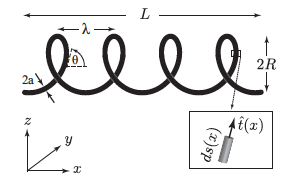
\includegraphics[width=0.7\textwidth]{parameters}
  \caption[Helix parameters]{The essential helix parameters to design a helical microrobot~\citep{rodenborn2013propulsion}.}
  \label{parameters}
%\end{center}
%\end{wrapfigure}
\end{figure}



The flagella rotation at low Reynolds number exerts an axial thrust ($F$) and torque ($T$) related to the
rotation rate ($\omega$) and flagellum axial velocity ($\nu$). At the same time, fluids was exerted the force
 ($-F$) and the torque ($-T$) on the swimming microrobots~\citep{purcell1997efficiency}. The fluid dynamic 
govern by the Stokes equations (\ref{stokes_1}) in the low Reynolds regime;


\begin{equation}
  -\nabla{p}+ \eta\nabla^2{\nu}  = 0
\label{stokes_1}
\end{equation}

Where $\eta$ and $p$ are fluid dynamic velocity and pressure respectively. Therefore thrust ($F$) and 
torque ($T$) are linearly related to the $\nu$ and $\omega$ as there are no derivation of time in 
the equations \ref{stokes_1}. Thses linear relationship can be defined as follow;



\begin{equation}
  F  = A\nu + B\omega
\label{linear1}
\end{equation}

\begin{equation}
  T = C\nu + D\omega
\label{linear2}
\end{equation}


 Therfore, a matrix 
$\bigl(\begin{smallmatrix}
A&B\\ C&D
\end{smallmatrix} \bigr)$
 defined as propulsion matrix the
model to explain the flagellar swimming motion described by following equation~\citep{rodenborn2013propulsion}
as mentioned in the literature review earlier;
 

\[
\begin{bmatrix} F\\ 
T\end{bmatrix}  = \begin{bmatrix} A & B \\ 
C & D \end{bmatrix}  \begin{bmatrix} \nu
 \\ \omega
\end{bmatrix}
\]

The elements in the symetric $2\times2$ matrix (propulsive matrix) in the above equation only depends on 
flagellum geometry. The propulsive matrix elements can be computed by three methods called;
resistive force theory, slender body theory and regularized Stokeslet theory which are described in details in sections \ref{method3}, 
\ref{method1} and \ref{method2} respectively. 


\subsubsection{Resistive force theory for microrobot with two degree of freedom}\label{method3}



%\begin{figure}
%  \centering
\begin{wrapfigure}{r}{0.5\textwidth}
  \begin{center}
    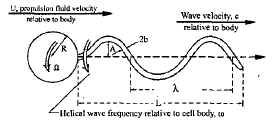
\includegraphics[width=0.5\textwidth]{motion}
  \caption[Microrobot filament motion]{Analysis of arbitary filament motion of microhelix~\citep{edd2003biomimetic}.}
  \label{motion}
\end{center}
\end{wrapfigure}
%\end{figure}



The swimming velocity and efficiency of the microrobot can be predicted by Resistive force theory (RFT)~\citep{purcell1997efficiency}. 
The force exerted on the fluid by micro swimmer were calculated initially and the micro swimmer will have a net 
movement if the force is not zero~\citep{Doe:2013:Online}. Furthermore, the swimming velocity will decrease if the helical
body attached to the innert head. Figure \ref{filament} shows an arbitary filament motion which is defined by $s(l,t)$. 
A direction of the helix velocity ($U$) is along x-axis and its rotation is symetric about the x-axis. 
The following assumption has been made in order to use the RFT. 

%\begin{figure}
%  \centering
\begin{wrapfigure}{r}{0.5\textwidth}
  \begin{center}
    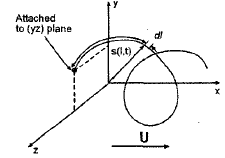
\includegraphics[width=0.5\textwidth]{filament}
  \caption[A motion of helical segment]{A motion of an arbitary filament~\citep{edd2003biomimetic}.}
  \label{filament}
\end{center}
\end{wrapfigure}
%\end{figure}


The geometry
of the helix is on the yz-plane and it always attached to the robot body (can be a sphere). The 
filament motion is periodic and filament length is constant at all the time. Acceleration can be neglected as the
system is in the low Re number fluid. Hence, the equations \ref{thrust_1} and \ref{torque_1} will describe the force balance and 
the moment balance in the x-axis direction. The thrust and torque will be determined by integrating over the 
first term of the force balance and moment balance equations (\ref{thrust_1} and \ref{torque_1}) 
 respectively ~\citep{edd2003biomimetic}.





\begin{equation}
  \cfrac {1} {\Delta T} \int_0^{\Delta T} \int_0^L  f_x(l,t)\: \mathrm{d}l \:\mathrm{d}t + C_DU  = 0
\label{thrust_1}
\end{equation}

\begin{equation}
  \cfrac {1} {\Delta T}  \int_0^{\Delta T} \int_0^L [\bold r \bold \times \bold f(l,t)] . \bold e_1x \: \mathrm{d}l \:\mathrm{d}t + C_{D\Omega}\Omega= 0
\label{torque_1}
\end{equation}

Where $\Delta T$ is the time filament motion repeats and integration is taken over the whole lenght $(L)$ of the
helix. 

\paragraph{}
In order to solve the integration problem, the force ($f$) is required to be defined. Therefore, a new
coordination system was introduced and the force vector was defined as a composition of force per unit length
in the normal and tangent directions. Two identical motions are considered for the swmming microrobots
are; rotating and translating (assumed in the x-axis direction). Hence, the force balance and moment balance 
equations are simplified as following; 


\begin{equation}
Nf_xL  + C_DU  = 0
\label{simple_thrust}
\end{equation}



\begin{equation}
 Nf_yAL + C_{D\Omega}\Omega= 0
\label{simple_torque}
\end{equation}

Where $N$ and $A$ are number of filaments and helical amplitude of filaments respectively. Also $f_x$ and 
$f_y$ shows the components of the force vector along x and y directions. In addition, $C_D$ and $C_{D\Omega}$
were computed by equations \ref{Coeff1} and \ref{Coeff2} where $R$ is redius of the helix and $\mu$ is fluid velocity.


\begin{equation}
 C_D  = 6 \pi \mu R
\label{Coeff1}
\end{equation}



\begin{equation}
 C_{D\Omega}= 8 \pi \mu R^3
\label{Coeff2}
\end{equation}

The $f_x$ and $f_y$ are written as composite of forces in the normal and tangent directions;

\begin{equation}
 f_x  = f_t\cos \theta - f_n\sin \theta
\label{normal}
\end{equation}



\begin{equation}
 f_y = f_t\sin \theta + f_n\cos \theta
\label{tangant}
\end{equation}

\begin{equation}
 \tan \theta  = \cfrac{\lambda}{2\pi A}
\label{tang}
\end{equation}



\begin{equation}
 f_t = -C_t(U \cos \theta - \omega A \sin \theta)
\label{normal_f}
\end{equation}



\begin{equation}
f_n = - C_n(-U \sin \theta - \omega A \cos \theta)
\label{tangant_f}
\end{equation}

Where $C_t$ and $C_n$ called resistance coefficients ~\citep{edd2003biomimetic};
 

\begin{equation}
 C_t = \cfrac{2 \pi \mu}{\ln (\cfrac{2 \lambda}{b}) - \cfrac{1}{2}}
\label{Coeffient1}
\end{equation}



\begin{equation}
 C_n = \cfrac{4 \pi \mu}{\ln (\cfrac{2 \lambda}{b}) + \cfrac{1}{2}}
\label{Coeffient1}
\end{equation}

Microrobot\rq{}s swimming speed and rotation rate were determined by solving 
the equations \ref{normal_f} and \ref{tangant_f}. Therefore, thrust ($F$), torque ($T$) and drag ($D$) 
on flagellum can be predict by following equations~\citep{rodenborn2013propulsion};

\begin{equation}
 F = (\Omega R)(C_n - C_t) \sin \theta \cos \theta \cfrac{L}{\cos \theta} 
\label{thrust}
\end{equation}

\begin{equation}
 T = (\Omega R^2)(C_n \cos ^2 \theta + C_t \sin ^2 \theta) \cfrac{L}{\cos \theta}
\label{torque}
\end{equation}

\begin{equation}
 D = U (C_n \sin ^2 \theta + C_t \cos ^2 \theta) \cfrac{L}{\cos \theta} 
\label{drag}
\end{equation}



Finally, the efficiency of the helical swimmers can be computed as follow;



\begin{equation}
 efficiency = \cfrac{FU}{T \omega} 
\label{efficiency}
\end{equation}

 
\subsubsection{Resistive force theory for six degree of freedom}\label{RFT_sixDegree}
 



The two degree of freedom microrobot (one dimention model) with \ac*{RFT} was exhibited a successful result~\citep{mahoney2011velocity}
for studying the helical microswimmers. However, complex motion of swimming microrobot could not been 
explained in one dimention model. Therefore, the \ac*{RFT} was needed to be implemented in three dimention
model which means defining a microrobot with six degree of freedom. The microrobot\rq{}s is
used in this model has a helical tail with the shpere head attached to it as shown in \ref{RFT-6dof}.

\begin{figure}
  \centering
%\begin{wrapfigure}{r}{0.5\textwidth}
%  \begin{center}
    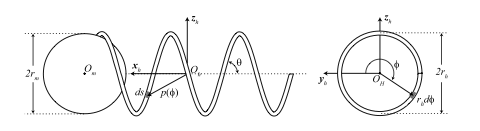
\includegraphics[width=1.0\textwidth]{RFT-6dof}
  \caption[Helical microrobot configration with a magnetic spherical head]{Three dimention configration for the helical microrobot with a magnetic spherical head. The origin
of the helix coordinate is denoted with $\bm{O}_h$ and $\bm{x}_{h}$ is the central axis of the
 helix~\citep{mahoney2011velocity}.}
  \label{RFT-6dof}
%\end{center}
%\end{wrapfigure}
\end{figure}

The \ac*{RFT} is applied with the assumption that the force and torue is applied on the helical tail and sphear
head are independent. Therefore, the force $f_h$ and torque $\tau_h$ of the helical tail are optained by \ac*{RFT} 
and $f_m$ and $\tau_m$ are force and torue are applied on the sphear head respectively. 
The equation \ref{total_force_torque} is the summation of two forces and torques which is the total force and torque. 

\begin{equation}
 f = f_h + f_m \qquad  \tau = \tau_h + \tau_m
\label{total_force_torque}
\end{equation}

According to the \ac*{RFT} the force on the extremely teeny segment of the helix is defined by 
the segment velocity and drag forces acts on that segment. First \ac*{RFT} takes the
 veloity ($\bm{V}_s$) was applied on the small length
of helix and decompound it into two vectors, one parallel ($\bm{V}_{\parallel}$) and one perpendicular ($\bm{V}_{\perp}$)
 to that segment. Also, the drag force is acting on that small length decomposed into two 
vectors; parallel (${\xi}_{\parallel}$) and perpendicular (${\xi}_{\perp}$) to that segment.  
Therefore, the force is applied on the small segment is formulated as follow; 

\begin{equation}
 d{\bm{f}_{\perp}} = {\xi}_{\perp}{\bm{V}_{\perp}}ds 
\label{relation-force_drag}
\end{equation}

\begin{equation}
 d{\bm{f}_{\parallel}} = {\xi}_{\parallel}{\bm{V}_{\parallel}}ds
\label{relation-force_drag}
\end{equation}

Where ${\xi}_{\parallel}$ and ${\xi}_{\perp}$ are drag coefficients and they have been approximated by number
of scientists emprically. The fluidic force ($ \bm{f}_h$) acts on the helix is computed by integrating over these 
differential forces along the helix length. Because the integration is performed in three dimention
 we need to define two seperate coordinate frame, one for the given
differential segment (frame $s$) and one for the helix (frame $h$). The helix pitch angle ($\theta$) 
and radius ($r_h$) is used to define the geometry of the helix with the assumption that the central
 axe of the helix is
parallel to the $\bm{x}_h$. Figure \ref{RFT-6dof} presents the helix coordinate origin ($O_h$) with 
its three axis ($\bm{x}_h , \bm{y}_h , \bm{z}_h$). The helix is represented in a cylindrical coordinate
\footnote{The cylindrical coordinate is an extention of the polar coordinate to the three dimention space. It
defines based on the radius $r$, the angle $\theta$ and the $z$ coordinate such that the following equation
are valid

\begin{equation}
 x = r\cos{\theta} \qquad  y = r\sin{\theta}  \qquad  z = z
\label{cylindrical_coordinate}
\end{equation}
}

system with the polar angle $\phi$. Each vector in the segment frame ($s$) can be written in the helix
frame ($h$) by applying a rotation matrix as shown in the equation \ref{rotation_matrix};
  

\begin{equation}
 ^{h}\bm{R}_s(\phi) = \bm{R}_x(\phi)\bm{R}_y(-\theta)
\label{rotation_matrix}
\end{equation}

Where $\bm{R}_x(\phi)$ is rotation of a vector in the segment frame ($s$) with the $\phi$ angle with
respect to the $x$
axis and then will apply $\bm{R}_y(-\theta)$ which rotate the result vector with the ($-\theta$) angle with
respect to the $y$ axis. The final result is a vector in the helix ($h$) frame \ref{rotated_vector}.



\begin{equation}
 ^{h}\bm{P}(\phi) = \begin{bmatrix}
       \frac{r}{\tan(\theta)} & r\cos(\phi) & r\sin(\phi)    \\[0.3em]
       
     			   \end{bmatrix}
\label{rotated_vector}
\end{equation}

Hence, as appears in the equation \ref{velocity_force_segment_frame} the differential relating velocity to force can be shown with respect to the frame of 
a random segment along the helix in the segment frame in three dimention.   



\begin{equation}
 ^{s}d\bm{f}_s = {^{s}\bm{\Xi}}{^{s}\bm{V}_s}{ds}
\label{velocity_force_segment_frame}
\end{equation}


\begin{equation}
 ^{s}\bm\Xi = \begin{bmatrix}
       \xi_{\parallel}  & 0 		 & 0           \\[0.3em]
       0		 & \xi_{\perp}           & 0\\[0.3em]
       0           	& 0 		& \xi_{\perp}
     \end{bmatrix}
\label{drag_coeffi_matrix}
\end{equation}

In the equation \ref{velocity_force_segment_frame} the force $^{s}\bm{f}_s$ and velocity $^{s}\bm{V}_s$ of
the segment is represented in the segment\rq{}s own frame. 
In the segment frame, the $x_s$ axis is assumed to be parallel to that segment and two other axis 
($y_s$, $z_s$) are perpendicular to that segment as we can see in the \ref{drag_coeffi_matrix}.
Hence, the relationship between forces and velocity can be expressed in the helix 
frame (\ref{velocity_force_helix_frame}) by using the drag coeffient unity matrix \ref{drag_coeffi_matrix}.

\begin{equation}
 ^{h}d\bm{f}_s = {^{h}\bm{\Xi}}(\phi){^{h}\bm{V}_s}{ds}
\label{velocity_force_helix_frame}
\end{equation}

where


\begin{equation}
{^{h}\bm{\Xi}}(\phi) = ^{h}\bm{R}_s(\phi){^{s}\bm{\Xi}}{^{s}\bm{R}_h(\phi)}
\label{drag_coeff_matrix_rotated}
\end{equation}

The velocity of the small helix segment $\bm{V}_s$ is formed of the rotational helix velocity ($\omega$) 
and its translational velocity ($\bm{V}$). The summation of two velocities is described in the equations
\ref{total_velocity}.

\begin{equation}
\bm{V}_s = \bm{V} + \bm{\omega} \times {\bm{P}(\phi)} = \bm{V} - {\bm{P}(\phi)}\times{\bm{\omega}}
\label{total_velocity}
\end{equation}

The equation \ref{total_velocity} is the velocity of the segment in the segment frame. 
This equation can be written with respect of the helix frame, as shown below;

\begin{equation}
^{h}\bm{V}_s = ^{h}\bm{V} - \Delta{\{^{h}\bm{P}(\phi)}\}^{h}\bm{\omega} = ^{h}\bm{V} + \Delta{\{^{h}\bm{P}(\phi)}\}^{Th}\bm{\omega}
\label{total_velocity_helixFrame}
\end{equation}

where the vector cross product (${\bm{P}(\phi)}\times{\bm{\omega}}$) can be represented in the form 
of skew-symmetric
martix \footnote{In mathematics, a square matrix $A$ is called a skew-symmetric if its transpose
is equal to its negative ($A^{T} = -A$).} $\Delta{\{^{h}\bm{P}(\phi)}\}^{h}$ and a vector
$\bm{\omega}$:

\begin{equation}
{\bm{P}(\phi)}\times{\bm{\omega}} = \Delta{\{^{h}\bm{P}(\phi)}\}^{h}{\bm{\omega}}
\label{cross_product}
\end{equation}

And acording to the skew-symmetric matrix property we have:

\begin{equation}
-\Delta{\{^{h}\bm{P}(\phi)}\}^{h} = \Delta{\{^{h}\bm{P}(\phi)}\}^{Th}
\label{skew_symetric_vector}
\end{equation}

After substituting \ref{total_velocity_helixFrame} into \ref{velocity_force_helix_frame}:

\begin{equation}
 ^{h}d\bm{f}_s = {^{h}\bm{\Xi}}(\phi){^{h}\bm{V}}{ds} + ^{h}\Xi(\phi)\Delta{\{^{h}\bm{P}(\phi)}\}^{Th}\omega{ds}
\label{Final_force_related_RotationTranslation}
\end{equation}

The equation \ref{Final_force_related_RotationTranslation} manifests the relation between differential force
and translation and rotation velocity of the small helix segment in the helix frame. Each force is applyed on 
an infinitesimally small section of helix generates a torque around helix centre. As a result the 
relation between the force and torque at an arbitary slice of helix (using parameter $\phi$) can be 
represented in the helix frame:

\begin{equation}
 ^{h}d\bm{\tau}_s = {^{h}\bm{P}(\phi)} \times ^{h}d\bm{f}_s=\Delta{\{^{h}\bm{P}(\phi)}\}^{h}{d\bm{f}_s}
\label{forceTorque_relation_helixFrame}
\end{equation}

Therefore the total fluidic torque and force of the helix can be figured out by integrating the small torques
and forces that applied on the infinitestimally segments of the helix along the helix length:

\begin{equation}
 \bm{f}_h = \int \; d\bm{f}_s  \qquad  \bm{\tau}_h = \int \; d\bm{\tau}_s 
\label{total_force_torque}
\end{equation} 
 
The final torque and force can be obtained from the equations \ref{total_force_torque} by 
integraling with respect to the polar angle $\phi$. As it been seen in the figure \ref{RFT-6dof} the $ds$
can be written with respect with the polar angle $\phi$ as follow:


\begin{equation}
ds = \frac{r_hd\phi}{\sin(\theta)}
\label{polar_angle_theta}
\end{equation} 

after substitiuting the \ref{Final_force_related_RotationTranslation} into \ref{forceTorque_relation_helixFrame} and 
replacing $ds$ with the eqation \ref{polar_angle_theta} we have the following equations which is 
integrating with respect with $\phi$ from $-\pi n$ to $\pi n$ for an $n$ turn helix;

 
\begin{multline}
\qquad \qquad^{h}\bm{f}_h = \left (  \frac{r_h}{\sin(\theta)}  \int _{-\pi n}^{\pi n} \mathrm {^{h}\Xi(\phi)}\, d(\phi)  \right){^{h}{\bm{V}}} \\ 
+ \left ( \frac{r_h}{\sin(\theta)}  \int _{-\pi n}^{\pi n} \mathrm {^{h}\Xi(\phi)}  \Delta{\{^{h}\bm{P}(\phi)}\}^T    \, d(\phi)    \right){^{h}{\bm{\omega}}}
\label{first_intergra_force}
\end{multline} 


\begin{multline}
\qquad \qquad ^{h}\bm{\tau}_h = \left (  \frac{r_h}{\sin(\theta)}  \int _{-\pi n}^{\pi n} \mathrm \Delta{\{^{h}\bm{P}(\phi)}\} {^{h}\Xi(\phi)}\, d(\phi) \right){^{h}{\bm{V}}} \\
 + \left ( \frac{r_h}{\sin(\theta)} \int _{-\pi n}^{\pi n} \mathrm \Delta{\{^{h}\bm{P}(\phi)}\} {^{h}\Xi(\phi)} \Delta{\{^{h}\bm{P}(\phi)}\}^T \, d(\phi) \right){^{h}{\bm{\omega}}}
\label{second_integral_torque}
\end{multline} 

Computing all four integrals in the eqations \ref{first_intergra_force} and \ref{second_integral_torque} will
result in two eqations that is expressed force $(^{h}\bm{f}_h)$ and torque $(^{h}\bm{\tau}_h)$ in 
terms of the anqular $(^{h}\bm{\omega})$ and translational velocity $(^{h}\bm{V})$: 


\[
\begin{bmatrix} ^{h}\bm{f}_h\\ 
^{h}\bm{\tau}_h\end{bmatrix}  = \begin{bmatrix} ^{h}\bm{A}_h & ^{h}\bm{B}_h \\ 
^{h}\bm{C}_h & ^{h}\bm{D}_h \end{bmatrix}  \begin{bmatrix} ^{h}\bm{V}_h
 \\ ^{h}\bm{\omega}
\end{bmatrix}
\]


Where $^{h}\bm{A}_h$, $^{h}\bm{B}_h$ and $^{h}\bm{C}_h$ are:

\begin{equation}
 ^{h}\bm{A}_h = \begin{bmatrix}
       a_{h11}  & 0 		 & 0           \\[0.3em]
       0		 & a_{h22}           & 0\\[0.3em]
       0           	& 0 		& a_{h22}
     \end{bmatrix}
\label{Amatrix}
\end{equation}


\begin{equation}
 ^{h}\bm{B}_h = \begin{bmatrix}
       b_{h11}  & 0 		 & b_{h13}          \\[0.3em]
       0		 & b_{h22}           & 0\\[0.3em]
       0           	& 0 		& b_{h33}
     \end{bmatrix}
\label{Bmatrix}
\end{equation}



\begin{equation}
 ^{h}\bm{C}_h = \begin{bmatrix}
       c_{h11}  & 0 		 & c_{h13}            \\[0.3em]
       0		 & c_{h22}           & 0\\[0.3em]
       c_{h13}            	& 0 		& c_{h33} 
     \end{bmatrix}
\label{Cmatrix}
\end{equation}


and each matrix element will calculate by following eqations:



\begin{equation}
a_{h11} = \frac{2\pi n r_h (\xi_{\parallel} \cos^2(\theta) + \xi_{\perp} \sin^2(\theta))}{\sin(\theta) }
\label{ah11}
\end{equation} 

\begin{equation}
a_{h11} = \frac{\pi n r_h (\xi_{\perp} + \xi_{\perp} \cos^2(\theta) + \xi_{\parallel} \sin^2(\theta))}{\sin(\theta) }
\label{ah22}
\end{equation} 

\begin{equation}
b_{h11} = 2\pi n {r_h}^2 (\xi_{\parallel} - \xi_{\perp})\cos(\theta)
\label{bh11}
\end{equation} 


\begin{equation}
a_{h13} = \frac{-2 \pi n {r_h}^2 (\xi_{\parallel} - \xi_{\perp})\cos(\theta)}{\tan(\theta) }
\label{bh13}
\end{equation} 


\begin{equation}
a_{h22} = \frac{-3 \pi n {r_h}^2 (\xi_{\parallel} - \xi_{\perp})\cos(\theta)}{2}
\label{bh22}
\end{equation} 


\begin{equation}
a_{h33} = \frac{- \pi n {r_h}^2 (\xi_{\parallel} - \xi_{\perp})\cos(\theta)}{2}
\label{bh33}
\end{equation} 



\begin{equation}
c_{h11} = \frac{2\pi n {r_h}^3 (\xi_{\perp} \cos^2(\theta) + \xi_{\parallel} \sin^2(\theta))}{\sin(\theta) }
\label{ch11}
\end{equation} 


\begin{equation}
c_{h11} = \frac{-2\pi n {r_h}^3 (\xi_{\perp} \cos^2(\theta) + \xi_{\parallel} \sin^2(\theta))}{\sin(\theta) \tan(\theta)}
\label{ch13}
\end{equation}


\begin{multline}
c_{h22} = \frac{2\pi n {r_h}^3 (\xi_{\parallel} \cos^2(\theta) + \xi_{\perp} \sin^2(\theta) - \xi_{\perp}/2)}{\sin(\theta) } \\
+ \frac{\pi n {r_h}^3 (\xi_{\parallel} \cos^2(\theta) - \xi_{\perp} \sin^2(\theta) - \xi_{\perp})}{2{\tan^2(\theta)}\sin(\theta)}\\
+ \frac{(\pi n {r_h})^3 (\xi_{\parallel} \cos^2(\theta) - \xi_{\perp} \sin^2(\theta) + \xi_{\perp})}{3{\tan^2(\theta)}\sin(\theta)}
\label{ch22}
\end{multline}



\begin{multline}
c_{h33} = \frac{\pi n {r_h}^3 \xi_{\perp} }{\sin(\theta) }- \frac{\pi n {r_h}^3 (\xi_{\perp} \cos^2(\theta) + \xi_{\parallel} \sin^2(\theta) - \xi_{\perp})}{2{\tan^2(\theta)}\sin(\theta)}\\
+ \frac{(\pi n {r_h})^3 (\xi_{\perp} \cos^2(\theta) + \xi_{\parallel} \sin^2(\theta) + \xi_{\perp})}{3{\tan^2(\theta)}\sin(\theta)}
\label{ch33}
\end{multline}


We assumed the fluidic torque and force are applied on microrobot by helical tail is independent from the
spherical head. We define a vector $\bm K$ such that it connects the centre of the helix $\bm O_h$ to the 
centre of the spherical magnetic head $\bm O_m$ as shown in the Figure~\ref{RFT-6dof}. The well-known
equations for the rotational and translational drag coefficient of the sphear particle in the stokes flow 
 are \citep{white1991viscous}:


\begin{equation}
\xi_{vm} = 6 \pi \eta r_m \qquad \qquad \xi_{\omega m} = 8 \pi \eta r^3_m
\label{shearical_drag_coefficients}
\end{equation}


Where $\eta$ is the fluid viscosity and $r$ is the radius of the sphear. A magnet velocity is produced by an 
arbitrary movement of the microswimmer and can be expressed in the helix frame as the product of the
head\rq{}s velocity and translational drag coefficient:


\begin{equation}
^{h}\bm V_{m} = ^{h}\bm{V} + ^{h}\bm{\omega} \times ^{h}\bm{ K }= ^{h}\bm {V} - ^{h}\bm{K} \times ^{h}\bm{\omega}
= ^{h}\bm{V} + \Delta \{^{h}\bm{ K} \}^{Th} \bm{\omega}
\label{magnet_velocity}
\end{equation}

Also, force on the spherical magnet is the product of the translational and rotational force:

 
\begin{equation}
^{h}\bm{f}_{m} = \xi_{vm} {^{h}{\bm{V}}} + \xi_{vm} \Delta\{ {^{h}\bm{K}}\}^{Th} \bm{\omega}
\label{magnet_force}
\end{equation}

The force acts at the arm $\bm{K}$ and the drag is generated by the rotation of the spherical magnet will 
couse a drag torque by magnet head:

 \begin{equation}
^{h}\bm{\tau}_{m} = ^{h}\bm{K} \times  ^{h}\bm{f}_{m} + \xi_{\omega m} {^{h}\bm{\omega}}
\label{magnet_head_torque}
\end{equation}

After replacing $^{h}\bm{f}_{m}$ with \ref{magnet_force} and using scew-symmetric matrix instead of
cross-product, the final torque for magnetic head will be:

 

\begin{equation}
^{h}\bm{\tau}_{m} = \xi_{vm}\Delta\{ {^{h}\bm{K}}\} {^{h}{\bm{V}}} + (\xi_{vm} \Delta\{ {^{h}\bm{K}}\}   {\Delta\{ {^{h}\bm{K}}\}}^{T} + \xi_{\omega m}  \bm{I} ){^{h}\bm{\omega}}
\label{magnet_torque_final}
\end{equation}


We can write the equation \ref{magnet_torque_fina} in terms of matrices;


\begin{equation}
^{h}\bm{A}_m = \xi_{vm} \bm{I}  \qquad  ^{h}\bm{B}_m = \xi_{vm} \Delta \{ ^{h}\bm{K} \}^T \qquad
{^{h}\bm{B}_m = \xi_{vm} \Delta \{ ^{h}\bm{K} \} \Delta \{ ^{h}\bm{K} \}^T} + \xi_{\omega m} \bm{ I}
\label{A_m}
\end{equation}

Therefore, the total torque ($^{h}\bm{\tau} =^{h}\bm{\tau}_h +^{h}\bm{\tau}_m$) and force
 ($^{h}\bm{f} =^{h}\bm{f}_h +^{h}\bm{f}_m$) applied on microswimmer are:


\[
\begin{bmatrix} ^{h}\bm{f}\\ 
^{h}\bm{\tau}\end{bmatrix}  = \begin{bmatrix} ^{h}\bm{A} & ^{h}\bm{B}\\ 
^{h}\bm{B}^{T} & ^{h}\bm{C} \end{bmatrix}  \begin{bmatrix} ^{h}\bm{V}
 \\ ^{h}\bm{\omega}
\end{bmatrix}
\]

By replacing the matrices with their equvalent;

%\begin{equation}
\[
\begin{bmatrix} ^{h}\bm{f}\\ 
^{h}\bm{\tau}\end{bmatrix}  = \begin{bmatrix} ^{h}\bm{A}_{h} + ^{h}\bm{A}_{m} & {^{h}\bm{B}_{h} + ^{h}\bm{B}_{m} }\\ 
({^{h}\bm{B}_{h} + ^{h}\bm{B}_{m} })^{T} & ^{h}\bm{C}_{h} + ^{h}\bm{C}_{m} \end{bmatrix}  \begin{bmatrix} ^{h}\bm{V}
 \\ ^{h}\bm{\omega}
\end{bmatrix}
\]
%\label{FINAL_PROPULSION}
%\end{equation}



\begin{equation}
 ^{h}\bm{A} = \begin{bmatrix}
       a_{11}  & 0 		 & 0           \\[0.3em]
       0		 & a_{22}           & 0\\[0.3em]
       0           	& 0 		& a_{22}
     \end{bmatrix}
	=
	 \begin{bmatrix}
       a_{h11}+\xi_{vm}  & 0 		 & 0           \\[0.3em]
       0		 & a_{h22}+\xi_{vm}           & 0\\[0.3em]
       0           	& 0 		& a_{h22}+\xi_{vm}
     \end{bmatrix}
\label{A_finalmatrix}
\end{equation}


\begin{equation}
 ^{h}\bm{B} = \begin{bmatrix}
       b_{11}  & 0 		 & b_{13}        \\[0.3em]
       0		 & b_{22}           & b_{23}\\[0.3em]
       0           	& -b_{23}		& b_{33}
     \end{bmatrix}
	=
	  \begin{bmatrix}
       b_{h11}  & 0 		 & b_{h13}          \\[0.3em]
       0		 & b_{h22}           & \xi_{vm}|\bm{K}|       \\[0.3em]
       0           	& - \xi_{vm}|\bm{K}| 		& b_{h33}
     \end{bmatrix}
\label{B_finalmatrix}
\end{equation}




\begin{equation}
 ^{h}\bm{C} = \begin{bmatrix}
       c_{11}  & 0 		 & c_{h13}            \\[0.3em]
       0		 & c_{22}           & 0\\[0.3em]
       c_{h13}            	& 0 		& c_{33} 
     \end{bmatrix}
	=
	 \begin{bmatrix}
       c_{h11}+ \xi_{\omega m} & 0 		 & c_{h13}            \\[0.3em]
       0		 & c_{h22}+  \xi_{vm}|\bm{K}|^2 +\xi_{\omega m}          & 0\\[0.3em]
       c_{h13}            	& 0 		& c_{h33} + \xi_{vm}|\bm{K}|^2 +\xi_{\omega m}
     \end{bmatrix}
\label{C_Finalmatrix}
\end{equation}

Hence, the total nonfluidic force ($\bm{f}$) which produced as a result of gravity and total nonfluidic torque
($\bm{\tau}$) generated by magnetic field. Then, the next algorithm is implemented  to control velocity of the
microrobot with considering gravity will detail in \ref{Microrobot actutation}.





\subsubsection{Regularized Stokeslet method}\label{method2}

A regularization parameter can be used as a proxy for the body radius to minimise numerical errors
 in modelling a flagellum as a one dimentional filament in a low Reynolds~\citep{smith2009boundary}.
number fluids. The Regularized Stokeslet method (RSM) is one of the approch to solve the zero 
Reynolds number linear \lq{}Stokes flow\rq{} equations;



\begin{equation}
 \left.\begin{aligned}
        0 &= - \nabla p + \mu \nabla ^ 2 u + f \\
        0 &=\nabla . u
       \end{aligned}
 \right\}
 \qquad \text{Stokes flow equations}
\label{stokes}
\end{equation}

where $u$ (velocity), $p$ (pressure), $\mu $ (kinematic viscosity), and $f$ (force) are measured per unit
volume. The singular \lq{}Stokeslet\rq{} solution for the equations \ref{stokes} corresponds to the purely 
viscous component (point force) of the flow which was determined by moving sphere. 
The \lq{}Stokeslet\rq{} solution for unit force acts in the j-direction and concentrated at $\xi $, where $f$ is;
  

\begin{equation}
 f (x) = \delta (x - \xi) e_j 
\label{force}
\end{equation}

$\delta (x - \xi)$ is called Dirac delta distribution. The velocity in the i-direction driven by this force is defined
 as follow;


\begin{equation}
 S _{ij} \bm{(x , \xi)} = (\frac{\delta _{ij}}{r} + \frac{r_i r_j}{r^3})
\label{i-direction}
\end{equation}

Where $\delta _{ij}$ denotes Kronecker delta tensor, $r_i = x_i - \xi _i$ and $r^2 =| \bm{x}- \bm{\xi} |^2 = r_1 ^2 + r_2 ^ 2 + r_3 ^2$.
The flow concentrates at point $\bm \xi$ by the force $\bold F$ where $ \bm{f (x)} = \delta (\bm{x} - \bm{\xi) F}$.
The solution is given by finding the velocity $u_i(\bm x)$;

\begin{equation}
 u_i(x) =(\frac{1}{8 \pi \mu}) S_{ij}\bm{( x, \xi)} F_j
\label{velocity}
\end{equation}

The \ac*{RFT} and  \ac*{SBT} for modelling of flagellum driven 
flow were formed on the base of the Stokeslet~\citep{smith2009boundary}. These methods solved the 
three dimentinal flow problem with flexible boundaries without using direct computation for the differential
equations. Therefore, the provided solution are extremely efficient in terms of computational costs. The fluid
velocity was modeled by the following equation;
   


\begin{equation}
\bold {u(x)} =(\frac{1}{8 \pi \mu}) \int_S \mathrm \bm{f(\xi)} . \bm{S( x, \xi)}\, \mathrm{d}S_{\xi}
\label{fluid_velocity}
\end{equation}

Where $S$ is a collection of lines or surfaces of flagella, $\bm{f(\xi)}$ shows force per unit length or area.
$\bm{f(\xi)} dS_{\xi}$ denotes the force flagella body exerted on the fluid and $-\bm{f(\xi)} dS_{\xi}$ is the 
force fluid applies to the body. The flagella is represented by equation \ref{fluid_velocity} with the boundary
$S$ and parameter $\bm{\xi (s)}$ where $0 < s <1$ is scaled arclength parameter. However, the flow field
at any point $\bm{x} = \bm{\xi} (s)$ is sigular and the collection of points on the surface of the filament 
are required to calculate the force per unit length. The collection of points were replaced on a small distance 
from the centreline;

\begin{equation}
\bold {X(s_q)} = \bm{\xi}(s_q) + a(s_q) \bm{n}(s_q)
\label{centreline}
\end{equation}

where $a(s_q)$ is a radius of slender body and $\bm{n}(s_q)$ is a unit normal vector. Point distributions of 
Stokeslets at any point $x = \bm{\xi}_q$ and line distribution inside the notional surface
of the flagella are both singular. However, surface distributions of Stokeslets do not result in singular  velocity
 but it still require attentive numerical implementations \citep{smith2009boundary}. The \lq{regularized Stokeslet}\rq{}
 introduced an exact solution for the equations \ref{$stokes_reg$} to overcome these issues. 
This method used a cut off function ($\psi$) with a regularization parameter ($\epsilon$) to smooth point forces 
such that $\int_{R^3} \psi_{\epsilon} (\bm{x})\, \mathrm{d}V_x = 1$.



\begin{equation}
 \left.\begin{aligned}
        0 &= - \bm{\nabla} p + \mu \nabla ^ 2 \bm{u} + \bm{f} \psi_\epsilon (\bm{x} - \bm{\xi}), \\
        0 &=\bm{\nabla . u}
       \end{aligned}
 \right\}
 \qquad \text{Stokes flow equations with regularization parameter}
\label{stokes_reg}
\end{equation}

In RSM method, with a assumption of $\psi_{\epsilon}(\bm{x} - \bm{\xi}) := 15\epsilon^4 /8\pi \mu r_{\epsilon}^7$ 
and $r_{\epsilon} = \sqrt{r^2 + \epsilon ^2}$ the regularized Stokeslet velocity tensor measured by the the following:


\begin{equation}
 S _{ij}^{\epsilon} \bm{(x , \xi)} = \frac{\delta _{ij}(r^2 + 2{\epsilon}^2) + r_i r_j}{r_{\epsilon}^3}
\label{velocity-tensor}
\end{equation}

Therefore the boundary for intergal equation (\ref{fluid_velocityReg}) is defined and the fluid velocity at location $x$ is;

\begin{equation}
\bold {u(x)} =(\frac{1}{8 \pi \mu}) \int_S \mathrm \bm{f(\xi)} . \bm{S^{\epsilon}( x, \xi)}\, \mathrm{d}S_{\xi}
\label{fluid_velocityReg}
\end{equation}

Where 



\subsubsection{Slender body theory}\label{method1}

Slender body theory represents the helix body with an arrangement of
 doublets and Stokeslets along the filament central line (Figure \ref{Stoks}). This theory represented by 
Lighthill for the first time and was followed by Johnson with some modification. According to \citeauthor{lighthill1971large}
there is some distance $q$ from any given point on the helix body such that $q$ is between the radius of the
filament $a$ and helix pitch $\lambda$. The dipoles is fallen within this distance are important to determine the flow at the
given point. He proved for the induced fluid flow on the given segment 
the sum of near-field and far-field solutions could be made independent of any distance ($q$) by definding
the dipoles as follow;

  

\begin{equation}
-\frac{a^2 \bm{f}_\perp (s)}{4\mu}
\label{dipole}
\end{equation}

Where $s$ is a location along the central axis of the filament and $\bm{f}_\perp (s)$ is Stokeslets strength\rq{}s
component which i perpendicular to the filament central axis. Therefore the sum of dipole and Stokeslets
define the flow induce by each segnment of the helix body. As a result there is a relation between 
the local velocity of a segment on the $s$ location and the force per unit length;



\begin{figure}
  \centering
%\begin{wrapfigure}{r}{0.5\textwidth}
%  \begin{center}
    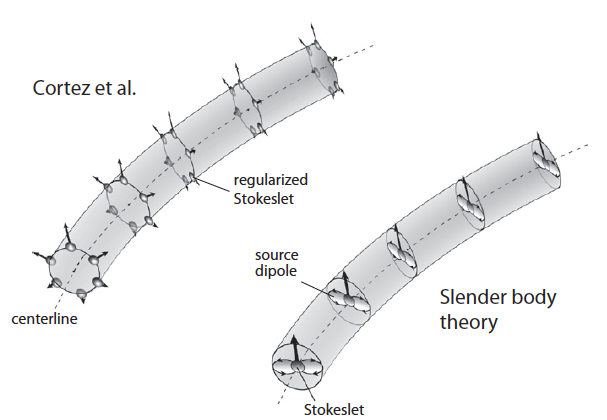
\includegraphics[width=1.0\textwidth]{Stoks}
  \caption[RSM and SBT]{\ac*{RSM} and \ac*{SBT}. In \ac*{RSM} the surface of helix filament separated by 
cross-sectional segmentation and each surface represents by 
Stokeslets (left image). In the \ac*{SBT}, the Stokeslets are arranged along the 
central filament line (rigth image)~\citep{rodenborn2013propulsion}.}
  \label{Stoks}
%\end{center}
%\end{wrapfigure}
\end{figure}




\begin{equation}
 \bm{u}(s) = -\frac{a^2 \bm{f}_\perp (s)}{4\mu} + \int_{|\bm{r_0}(s\rq{},s)| > \delta } \bm{f}(s\rq{}).J(\bm{r_0})\: \mathrm{d}s\rq{}
\label{dipole_stokes}
\end{equation}



Where $\bm{r_0}$ is the vector from the point $s$ on the central axis to the point $s\rq{}$ and $\delta$ is
 a natural cutoff ($\delta = \frac{a\sqrt{e}}{2}$). For the spatial location $r$ Oseen tensor $J$ is;

 
\begin{equation}
 J(\bm{r}) \equiv \frac{1}{8\pi \mu} (\frac{I}{|\bm{r}|} + \frac{\bm{rr}^T}{|\bm{r}|^3})
\label{Oseen}
\end{equation}

The thrust, torque and drag of the helical microswimmer can be optained by applying rectangular rule of
numerical integration and as a result we have;


\begin{equation}
 J(\bm{r}) \equiv \frac{1}{8\pi \mu} (\frac{I}{|\bm{r}|} + \frac{\bm{rr}^T}{|\bm{r}|^3})
\label{Oseen}
\end{equation}

We need to parameterize spatial locations, so we define helical phase $\phi \equiv ks \cos(\theta)$ where 
$k = 2 \pi / \lambda$ and $\bm{r} = R(\phi \cot(\theta), \cos(\phi) , \sin(\phi))$. Therefore equation \ref{dipole_stokes}
is converted to following equation;




\begin{equation}
\bm{u}_n = \frac{(I- \hat{t}_n\hat{t}_n + D_n). \bm{f}_n}{4\pi \mu}
+ \frac{\bm{R}\bm{\Delta}\phi \csc (\theta)}{8 \pi \mu} \sum_{m \neq n}  \frac{I+\hat{r}_{nm} \hat{r}_{nm}}{r_{nm}}. \bm{f}_m
+ \Lambda (\Delta \phi)
\label{numerical}
\end{equation}




Where $m,n = 1,2, \dots ,N$ and $\hat{t}_n=(\cos(\theta), -\sin(\theta)\sin(\phi_n), \sin(\theta)\cos(\phi_n))$.
The position vector between spatial location is $\bm{r}_{nm} = \bm{r}(\phi_n)- \bm{r}(\phi_m)$.

The components of the velocity $\bm{u}_n$ that are invariant alongside the helix can be obtained by 
integrating over the eqation \ref{numerical} and using the frame rotated with the helical phase. Then we can
find the linear mapping between force and velocity per unit length and calculate rotational and translation velocity
to find the force, torque and drag.

The first part of the equation \ref{numerical} is called tensor $D_n$ and it shows the helical segments that
are centered at $\bm{r}$. $D_n$ can be expressed in the form of following integral;


\begin{equation}
D_n = 1/2 \int_{|\bm{r}-\bm{r_n}| \in (\delta, \delta \rq{})} ds(\phi) \big(\frac{I}{|\bm{r}-\bm{r}_n|} + \frac{(\bm{r} -\bm{r}_m)(\bm{r} -\bm{r}_m)}{|\bm{r}-\bm{r}_n|^3} \big). \chi_z(\phi-\phi_n)
\label{functionD}
\end{equation}


Where the rotation matrix $\chi_z$ is defined as;



\begin{equation}
  \chi_z = \begin{bmatrix}
       \cos(\phi)  &  -\sin(\phi) 		 & 0           \\[0.4em]
       \sin(\phi)		 & \cos(\phi)           & 0\\[0.4em]
       0           	& 0 		&  1
     \end{bmatrix}
\label{rotationOperator}
\end{equation}

We define new vectors for force and velocity to simplify the calculation;



\begin{equation}
{\bm{u}_n}\rq{}= \chi_z(-\phi_n). \bm{u}
\label{NewVelo}
\end{equation}

\begin{equation}
{\bm{f}_n}\rq{}= \chi_z(-\phi_n). \bm{f}
\label{NewForce}
\end{equation}

Therefore the velocity ${\bm{u}_n}\rq{}$ is invariant to the filament and the rotational and translational velocity 
of the helix can be written as;

\begin{equation}
{\bm{u}_n}\rq{}= (0, \bm{\Omega} \bm{R} , \bm{U})^T
\label{NewVelo1}
\end{equation}

And the force;


\begin{equation}
\sum_{i=1} {\bm{f}}\rq{} \bm{R} \bm{\Delta}\phi \csc \theta = {\big(0, \bm{T}/\bm{R}, \bm{F}_x \big)}^T
\label{Newforce1}
\end{equation}

Therefore \ac*{SBT} can be expressed as;

\begin{multline}
\qquad {\bm{u}_n}\rq{}= \frac{(I- \hat{t}_n\hat{t}_n + D_n). \bm{f}_n}{4\pi \mu}\\
+ \frac{\bm{R}\bm{\Delta}\phi \csc (\theta)}{8 \pi \mu} \sum_{m \neq n}  \frac{ \chi_z(\phi_m - \phi_n)+ \chi_z(-\phi_n).\hat{r}_{nm}\hat{r}_{nm}. \chi_z(-\phi_n)}{r_{nm}}. {\bm{f}_m}\rq{}\\
+ \Lambda (\Delta \phi) \qquad \qquad \qquad \qquad \qquad \qquad \qquad \qquad \qquad \qquad
\label{NewVelo2}
\end{multline} 



Where both ${\hat{t}}\rq{}$ and ${D_n}\rq{}$ are invariant to the helical filament,


\begin{equation}
{\hat{t}}\rq{}= (0, \sin \theta, \cos \theta)
\label{invariant}
\end{equation}


and 


\begin{equation}
\int_{k \delta \cos \theta}^{k {\delta}\rq{} \cos \theta} \mathrm  d\phi \frac{1}{\phi}(I +\begin{pmatrix}
  0 & 0 & 0 \\
  0 & \sin^2\theta  & \sin\theta\cos\theta \\
  0 & \sin\theta\cos\theta & \cos^2\theta
 \end{pmatrix})=\ln(\frac{\delta\rq{}}{\delta})(I + {\hat{t}}\rq{} {\hat{t}}\rq{})
\label{FinalD}
\end{equation}


So we obtained the mapping between the force and velocity;



\begin{equation}
\begin{pmatrix}
  {\bm{u}_1}\rq{}  \\
  {\bm{u}_2}\rq{} \\
  \vdots  \\
   {\bm{u}_N}\rq{} 
 \end{pmatrix} = \Delta . \begin{pmatrix}
  {\bm{f}_1}\rq{}  \\
  {\bm{f}_2}\rq{} \\
  \vdots  \\
   {\bm{f}_N}\rq{} 
 \end{pmatrix}
\label{mapping}
\end{equation}


For the velocity ${\bm{u}_n}\rq{} = {\bm{u}_0} = (0, \bm{\Omega} \bm{R}, \bm{U})^T$ we have;



\begin{equation}
\begin{pmatrix}
  {\bm{f}_1}\rq{}  \\
  {\bm{f}_2}\rq{} \\
  \vdots  \\
   {\bm{f}_N}\rq{} 
 \end{pmatrix} = {\Delta}^{-1}. \begin{pmatrix}
  {\bm{u}_0}  \\
  {\bm{u}_0} \\
  \vdots  \\
   {\bm{u}_0} 
 \end{pmatrix}
\label{mappingInverse}
\end{equation}


Finally, the fluidic force and torque are;



\begin{equation}
 (0, \frac{T}{R}, F_x)^T = \sum_{i=1}^{N} \bm{f}\rq{} \bm{R} \bm{\Delta}\phi \csc \theta
\label{torqForce}
\end{equation}













\subsection{Microrobot actutation}\label{microActuation}



%\subsubsection{Force driven microrobot}

%\subsubsection{Torque driven microrobot}

In this section the aim is to develop an algorithm for the microrobot velocity control. To achive that, we need to 
fiqure out the direction that microrobot points out $(\bm{X}_{h})$ and then its rotational speed $(\Omega)$
 to obtain a desired velocity \cite{mahoney2011velocity}.
In this algorithm, the only nonfluidic force is applied on the microrobot is its weight which expressed as 
$m\bm{g}$. The mass of the microrobot is $m$ and the vector $\bm{g}$ shows the acceleration gravity. 
The direction of the gravity is downward and represented by $\hat{ \bm{g} }= \bm{g}/ \| \bm{g}\|$.




%%%%%%%%%%%%%%% Flochart of the control algorithm %%%%%%%%%%%%


Flowchart for Algorithm of the actuation method

%%%%%%%%%%%%

Previous research on controlling a microswimmers\rq{}s speed is evident that there is a lack
of control if commanding microrobot with too rapid maneuvers \citep{zhang2009characterizing} \citep{zhang2009artificial}
. Therefore, in this work we assumed
microswimmers can turn continuously to the aimed direction in such away that the temporary behavior is been
ignored. We define $\tilde{\bm{X}}$ as the axis magnetic field should always be perpendicular to it.
If the microrobot coordinate frame is aligned with the stationary world frame then there it does not require
to convert vectors between these two frames. From the helical propulsion equation system, 
we specifically considering the first equation which is the relation between non-fluidic force, angular and 
translational velocity of the microswimmer. 



\begin{equation}
^{h}\bm{f} = ^{h}\bm{A} ^{h}\bm{V} + ^{h}\bm{B} ^{h}\bm{\omega}
\label{first_lineOf_ propulsion method}
\end{equation}

The matrix $^{h}\bm{A}$ is invertible, thus the desired velocity can be obtained from the
 equation \ref{first_lineOf_ propulsion method};


\begin{equation}
^{h}\bm{V} = (^{h}\bm{A} ^{-1}){^{h}\bm{f}} + (-^{h}\bm{A} ^{-1} {^{h}\bm{B}}){^{h}\bm{\omega}} = 
^{h}\bm{D} ^{h}\bm{f} + ^{h}\bm{E} ^{h}\bm{\omega}
\label{first_lineOf_ propulsion method2}  
\end{equation}


\begin{equation}
 ^{h}\bm{D}_h = \begin{bmatrix}
       d_{11}  & 0 		 & 0           \\[0.3em]
       0		 & d_{22}           & 0\\[0.3em]
       0           	& 0 		& d_{22}
     \end{bmatrix}
\label{Dmatrix}
\end{equation}




\begin{equation}
 ^{h}\bm{E}_h = \begin{bmatrix}
       e_{11}  & 0 		 & 0           \\[0.3em]
       0		 & e_{22}           & 0\\[0.3em]
       0           	& 0 		& e_{22}
     \end{bmatrix}
\label{Ematrix}
\end{equation}

The equations \ref{first_lineOf_ propulsion method2}, \ref{Dmatrix}, \ref{Ematrix} are in the helix frame and 
can be converted to the world frame by applying relation matrix $^{w}\bm{R}_h$ on the equation
\ref{first_lineOf_ propulsion method2};


\begin{equation}
{^{w}\bm{R}_h}{^{h}\bm{V} } = {^{w}\bm{R}_h}{ ^{h}\bm{D} ^{h}\bm{f}} + {^{w}\bm{R}_h}{^{h}\bm{E} ^{h}\bm{\omega}}
\label{first_lineOf_ propulsion method3}  
\end{equation}



\begin{equation}
^{w}\bm{V}  ={^{w}\bm{E}} {^{w}\bm{\omega}} + {^{w}\bm{D}} {^{w}\bm{f}}  
\label{first_lineOf_ propulsion method4}  
\end{equation}

Then by applying the similar transformation to other component \ref{Dmatrix}, \ref{Ematrix};

\begin{equation}
^{w}\bm{V}  = {^{w}\bm{R}_h}{^{h}\bm{V}}  \qquad  ^{w}\bm{f}  = {^{w}\bm{R}_h}{^{h}\bm{f}}
\qquad  ^{w}\bm{D}  = {^{w}\bm{R}_h}{^{h}\bm{D}} {^{h}\bm{R}_w}
\qquad  ^{w}\bm{E}  = {^{w}\bm{R}_h}{^{h}\bm{E}} {^{h}\bm{R}_w}
\label{first_lineOf_ propulsion method5}  
\end{equation}

 To obtain ${^{h}\bm{R}_w}$ the orientation of the microrobot is required to be detected 
whilst it is rotating during propulsion around the axis which is difficult. For that reason, the equation
\ref{first_lineOf_ propulsion method4} is expressed in such way that it does not require to know the
microrobot orientation whilst rotating about its central axis. Since the microrobot is torque driven and the only 
nonfoluidic force is involved in equation \ref{first_lineOf_ propulsion method} is its weight $(m \bm{g})$. The 
velocity of microrobot can be decomposed to vertical and horizantal components:

 \begin{equation}
\bm{V}_{ver} = (\bm{V . \hat{g}})\bm{\hat {g}}
\label{vertical_velo}
\end{equation}


\begin{equation}
\bm{V}_{hor} = \bm{V} - \bm{V}_{ver}  
\label{horiantal_velo}
\end{equation}

Two options can be considered for the ${\| \bm {{V}_{hor}}\|}$:


\begin{equation}
 {\| \bm {{V}_{hor}}\|}  = 0 \qquad ,  \qquad  {\| \bm{{V}_{hor}}\|} \neq 0
\label{total_force_torque}
\end{equation}

The first option is a trival case, because when the microrobot is being commanded with
$ {\| \bm {{V}_{hor}}\|}  = 0$, that means the microrobot only swim vertically in either 
directions according to the equasion \ref{horiantal_velo}. This is the spacial case when the six degree of
freedom microrobot will effevtively become the microrobot with two degree of freedom which is pointing
in the direction of the gravity acceleration and its angular velocity can be found directly from the eqation
\ref{first_lineOf_ propulsion method4}:


\begin{equation}
 \bm {\Omega}  = \frac{{\| \bm{V}\|}+ d_{11}\| \bm{f}\|}{e_{11}}  \qquad ,  \qquad  \tilde{\bm{X}} = -\hat{\bm{g}}
\label{angular_velo_horiVelo=0}
\end{equation}

The second option ${\| \bm{{V}_{hor}}\|} \neq 0$ is more challenging, because it is required to set 
the coordinate frame for microrobot which does not rotate when the it is rotating around the central axis.
The ideal coordinate frame can be constructed by using $\hat{\bm{g}}$ and based on the eigenvectors
\footnote{If we have a set of data point, the set can be deconstructed into eigenvector and eigenvalue
where eigenvector is the direction that data spread out and eigenvalue is the variance of the data in that
direction. The principle component is the eigen vector with the largest eigenvalue \citep{Doe:2013Oct:Online}.} of 
$^{w}\bm{D}$ or $^{w}\bm{E}$. This coordinate system is denoted by $p$ and can be defined as :


\begin{equation}
 \bm{x}_p = \frac{(\bm{{x}_h . V )x_h}}{|\bm{x_h .V}|}
\label{x_pAxis}
\end{equation}



\begin{equation}
 \bm{y}_p = \frac{(\bm{{x}_p \times g)}}{\| \bm{x_p \times g}\|} 
\label{y_pAxis}
\end{equation}


\begin{equation}
 \bm{z}_p = \bm{{x}_p \times {y}_p}
\label{z_pAxis}
\end{equation}


\begin{figure}
  \centering
%\begin{wrapfigure}{r}{0.5\textwidth}
%  \begin{center}
    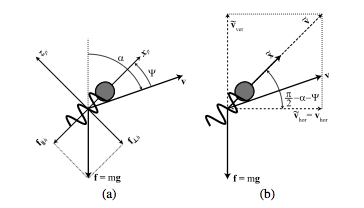
\includegraphics[width=1.0\textwidth]{horiz_verti_velocity}
  \caption[Construction details of 
direction of the microswimmer]{(a) The principle coordinate frame based on the gravity and principle componets
of the matrices in equations \ref{Ematrix} and \ref{Dmatrix}. (b) Construction details of 
direction of the microswimmer ($\bm{\tilde{X}}$)~\citep{mahoney2011velocity}.}
  \label{horiz_verti_velocity}
%\end{center}
%\end{wrapfigure}
\end{figure}

The new (principle) coordinate system will solve the problem because it is invariant to the rotation
 of the microswimer around its central axis. Therefore the equation \ref{first_lineOf_ propulsion method4} can
be expressed in terms of the principle coordinate frame. In the following paragraph
We first configure the representation for the first componet (${^{w}\bm{E}} {^{w}\bm{\omega}}$) of the 
equation \ref{first_lineOf_ propulsion method4} 
 and followed by similar process on the second componet (${^{w}\bm{D}} {^{w}\bm{f}}$). The final result will express the 
desired velocity vector in terms of the principal coodinate system. 


It is assumed that the microrobot is at steady state, that means $^{w}\bm{\omega} = 
\Omega \tilde{^{w}{\bm{x}}} = \Omega {^{w}{\bm{x}_p}}$, aslo we know two vectors ${^{w}{\bm{x}_p}}$ and
 ${^{w}{\bm{x}_h}}$ are parallel. It has been proved that $^{h}\bm{x}_h$ and $e_{11}$ are eigenvector and eigenvalue
of matrix $^{h}\bm{E}$ respectively \citep{mahoney2011velocity}. The transformation matrix $^{w}\bm{R}_h$ 
will not affect the eigenvalue ($e_{11}$) but it will rotate the eigenvector ($^{h}\bm{x}_h$) from the helix coordinate
frame to the global frame ($w$). As a result ($e_{11}$) and ($^{w}\bm{x}_p$) are the eigenvalue and eigenvector
in the world coordinate system respectively. By considering the vectors $^{w}\bm{x}_p$ and $^{h}\bm{x}_p$ are parallel 
and definition of eigenvalue and eigenvector \footnote{Assume $A $ is a square matrix $n \times n$, we call
$\lambda$ an eigenalue of matrix $A$ if the non-zero vector $\bm{V}$ exists such that $A\bm{V} = \lambda \bm{V}$.
The vector $V$ is called eigenvector corresponding to eigenvalue $\lambda$.
 \citep{Doe:2013Nov:Online}.}
the first componet of the desired velocity (${^{w}\bm{E}} {^{w}\bm{\omega}}$) can be 
represented in the principle
coordinate system as follow:


\begin{equation}
{^{w}\bm{E}} {^{w}\bm{\omega}} = {^{w}\bm{E}} \Omega {^{w}{\bm{x}_p}} = e_{11} \Omega {^{w}{\bm{x}_p}}
\label{E_W}
\end{equation}

The similar reasoning has been used to represent the second componet (${^{w}\bm{D}} {^{w}\bm{f}}$) of 
the velocity equasion (\ref{first_lineOf_ propulsion method4}) in terms of the
principle coordinate system. In this case, $d_{11}$ and $d_{22}$ are eigenvalues of the matrix $^{h}\bm{D}$ 
such that $^{h}\bm{x}_h$ is the eigenvector corresponding to the $d_{11}$ and $d_{22}$ is associated with
an eigenspace \footnote{Let $A $ be a $n \times n$ square matrix with an 
eigenvalue $\lambda$. Then the union of all eigenvectors associated with the eigenvalue $\lambda $ and
vector zero is a subspace of $\Re ^{3}$ which is called the eigenspace for the eigenvalue $\lambda$.
\citep{Doe:2014Aug:Online}.} spanned by $\{ ^{h}\bm{y}_{h} , ^{h}\bm{z}_{h} \}$. Again, the eigenvalues and
eigenspace will remain unaffected under transformation matrix. Thus, the eigenvalue $d_{11}$ is corresponding 
to the $^{w}\bm{x}_h$ and the eigenvalue $d_{22}$ is related to the vector in the 
subspace $\{ ^{w}\bm{y}_h ,   ^{w}\bm{z}_h  \}$. In addition the force vector can be decomposed into two  
vectors; one parallel to the central axis of helix and the other perpendicular to that axis ($^{w}\bm{x}_h$):



\begin{equation}
{^{w}\bm{f}} = \left ( (\bm{f} . \bm{x}_h) ^{w}\bm{x}_h \right) +  \left ( (\bm{f} . \bm{y}_h) ^{w}\bm{y}_h
 +  (\bm{f} . \bm{z}_h) ^{w}\bm{z}_h \right) = {^{w}\bm{f}}_{\parallel h} + {^{w}\bm{f}}_{\perp h}
\label{f_Component_globalAxis}
\end{equation}

If ${^{w}\bm{f}}_{\perp h}$ deos not change then both ${^{w}\bm{f}}$ and ${^{w}\bm{f}}_{\parallel h}$ will 
not change if microrobot rotate around its central axis. In addition, $^{w}\bm{y}_p$ and $^{w}\bm{z}_p$ are 
in the eigenspace formed by $\{ ^{w}\bm{y}_h ,   ^{w}\bm{z}_h  \}$. As a result, ${^{w}\bm{f}}_{\perp h}$ can be written in the 
principle coordinate frame as a linear combinations of two vectors ${^{w}\bm{z}}_{p}$ and 
${^{w}\bm{y}}_{p}$. Beacuse $d_{22}$ is the corresponding eigenvalue of any vector in the span of the
 $\{ ^{w}\bm{y}_h , ^{w}\bm{z}_h  \}$, so it will be the eigenvalue associated with ${^{w}\bm{f}}_{\perp h}$.
Using the fact that $d_{11}$ is the eigenvalue corresponding to $ {^{w}\bm{f}}_{\parallel h} $ and implying 
the transformation matrix we can write the force based on the principle component axis:
   


\begin{multline}
\qquad \qquad     \qquad   {^{w}\bm{D}} {^{w}\bm{f}} = {^{w}\bm{D}} {^{w}\bm{f}}_{\parallel h} + {^{w}\bm{D}} {^{w}\bm{f}}_{\perp h}
= d_{11} {^{w}\bm{f}}_{\parallel h} + d_{22}  {^{w}\bm{f}}_{\perp h}\\ 
= d_{11} \left ({\bm{f} . {\bm{x}}_p   }  \right) {^{w}\bm{x}}_p + 
 d_{22} \left ({\bm{f} . {\bm{z}}_p   }  \right) {^{w}\bm{z}}_p  \qquad \qquad
\label{force_principle_Components}
\end{multline} 

Both components  of the desired velocity are written on the basis of the principle components.
By replacing equations \ref{E_W} and \ref{force_principle_Components} in equation \ref{first_lineOf_ propulsion method4} we have:



\begin{equation}
^{w}\bm{V}  =   d_{11} \left ({\bm{f} . {\bm{x}}_p   }  \right) {^{w}\bm{x}}_p + 
 d_{22} \left ({\bm{f} . {\bm{z}}_p   }  \right) {^{w}\bm{z}}_p + e_{11} \Omega {^{w}{\bm{x}_p}}
\label{velocity_based_principle}  
\end{equation}

Therefore, non of the component of the velocity will be change when microrobot rotates around the central
axis. 

Since ${\| \bm{{V}_{hor}}\|} \neq 0$, as it is shown in the Fig \ref{horiz_verti_velocity} we can define 
the angle $\alpha$ between the vector $\bm{v}$ and the vertical axis in the world frame.



\begin{equation}
\alpha = {\tan}^{-1} ({\| \bm{V}_{hor} \|} / {\| \bm{V}_{ver} \|})
\label{alpha_velocity}  
\end{equation}

The microrobot requires to be position above the desired velocity vector (upward) with the angle $\psi$ 
 to compensate for the gravity vector. If we project the the desired velocity equation (\ref{velocity_based_principle})
into principle coordinate axis then we have:


\begin{equation}
(\bm{V} . \bm{x}_p) = d_{11} \left ({\bm{f} . {\bm{x}}_p   }  \right) + e_{11} \Omega 
\label{Xp_velocity}  
\end{equation}




\begin{equation}
(\bm{V} . \bm{z}_p) = d_{22} \left ({\bm{f} . {\bm{z}}_p   }  \right)
\label{Xz_velocity}  
\end{equation}

As it can be seen in the Fig \ref{horiz_verti_velocity}, the both side of the 
equation \ref{Xz_velocity} can be replaced by its equivalents:


\begin{equation}
(\bm{V} . \bm{z}_p) = - {\| \bm{V} \|} \sin(\psi)
\label{Xz_velocity_equival}  
\end{equation}


\begin{equation}
(\bm{f} . \bm{z}_p) = {\| \bm{f} \|} \sin(\psi - \alpha)
\label{Xz_velocity_equivali}  
\end{equation}



Thus, the replacing will lead to the following:


\begin{equation}
 - {\| \bm{V} \|} \sin(\psi) = d_{22} {\| \bm{f} \|} \sin(\psi - \alpha)
\label{finding_psi}  
\end{equation}

by applying the subtraction law for $ \sin(\psi - \alpha)$ \footnote{$\sin(\psi - \alpha) = 
\sin(\psi) \cos(\alpha) - \cos(\psi) \sin(\alpha)$},
 the angle $\psi$ can be optained from the following
equation:


\begin{equation}
  {\psi} ={{\tan}^{-1}} 
\frac{\left( d_{22} {\| \bm{f} \|} \sin(\alpha) \right)}{ \| {\bm{V} \| + d_{22} \| {\bm{f}} \|} \cos(\alpha) }
\label{psi}  
\end{equation}


All the parameters in the above equation are known and the direction point ($\tilde{\bm{X}}$) of the microrobot
 can be reconstructed by using angles $\alpha$ and $\psi$ and defining a dummy vector $\tilde{\bm{V}}$ such
that $\tilde{\bm{V}} = {\tilde{\bm{V}}}_{ver} + {\tilde{\bm{V}}}_{hor} $ where 
${\tilde{\bm{V}}}_{ver} = - \| {\tilde{\bm{V}}}_{hor} \| \tan(\pi /2 - \alpha + \psi) \hat{\bm{g}}$ and 
${\tilde{\bm{V}}}_{hor}  = {{\bm{V}}}_{hor}$. Therefore the final solution for the direction point is:



\begin{equation}
 \tilde{\bm{X} }  = \frac{\tilde{\bm{V}}}{\| {\tilde{\bm{V}}} \|}
\label{direction_point}  
\end{equation}

Therefore the angular velocity ($\Omega$) will be derived from equation \ref{Xp_velocity}, considering that
$(\bm{V} . \bm{x}_p) = \| {\bm{V}} \|  \cos({\psi})$ and $({\bm{f} . {\bm{x}}_p  }) = - \| {\bm{f}} \| \cos(\psi - \alpha) $ :




\begin{equation}
 \Omega  = \frac{\| {\tilde{\bm{V}} \|  \cos(\psi) }   + d_{11}  \| \bm{f} \| \cos(\psi - \alpha)}{e_{11}}
\label{FinalAngular_velo}  
\end{equation}

At this point the rotational velocity of microrobot can be used to compute the magnetic torque according to
the following equasion from propulsion equasion system;


\begin{equation}
 \tau = \bm{B} \bm{V} + \bm{C} \Omega 
\label{finalTorque_rotation}  
\end{equation}

Where $\bm{V}$ is known and $\bm{B}$ and $\bm{C}$ are precomputed from coeffient matix. Then considering
  magnetic torque equasion and replacing torque by its equivalent \ref{finalTorque_rotation};

\begin{equation}
 \tau = \bm{V}M \times \bm{B}
\label{finding-B}  
\end{equation}

Where $M$ magnetisation constant and $V$ is a volume of the magnetic object. Finally, the electric current 
($i$) is required to generate a dynamic magnetic field is achieved by the following; 


\begin{equation}
|\bm{B}| = (\frac{b^2}{(b^2+l^2)^{3/2}}){\mu}_0 i
\label{Current}  
\end{equation}


And the simulation algorithm is completed.

\begin{comment}
%%%%%%%%%
%%%%%%%%%%%%%%%%%%%% Testing %%%%%%%%%%%%%
%%%%%%%%%
\chapter{Experiments}

% Table show the range of wireless microrobopts input frequency and their speed.

Fe-ABF and FeTi-ABFs 
two magnetic fields of strenghts 1mT and 3 mT
The test show that forward speed is increasing with increasing input frequency below a critical value
 called (step-out frequency is the maximum magnetic field frequency that the ABFs can follow synchronously).
The step out frequency increases with the strength of the magnetic field. the maximum speed of Fe-ABF was
48.9 $\mu ms^{-1}$ at the field strength of $9 mT$ and $72 Hz$ ~\citep{qiu2014noncytotoxic}.

\end{comment}

%%%%%%%%%
%%%%%%%%%%%%%%%%%%%% Results %%%%%%%%%%%%%
%%%%%%%%%
\chapter{Results}\label{result}

\section{Simulation}
The aim of implementing the simulation framework for microhelix is to analyze the effect of 
the key parameters on microhelix\rq{}s efficiency. Also, finding the force, torque and drag act on 
the body of the helix. As the microhelix is in a fluid environment, investigating the effect of swimming
 mechanism is another aspect of this implementation. Evaluating the outcome of using a different fluid 
environment is part of the simulation. 

\paragraph{Simulation software}
Initially, Matlab was selected as the simulator software. However, after exploring the different aspects
 of the simulation, it became evident that the limitations of the software made it impossible to develop a complete simulation
 framework. One of the limitations was the software inability to incorporate and bind all the physics involved in this simulation 
modeling. Furthermore, Matlab was incapable of considering all aspects of a fluid environment. Therefore, 
another simulation software called COMSOL was used to implement the model. Although, COMSOL offers 
many build in environment that helps to make our simulation model, implementing an entire framework was 
required many considerations. 

\paragraph{Model components}

 The system configration (figure \ref{Simulation framework}) is based on the experiment setup
run by \citeauthor{mahoney2011velocity} however they run an experiment on a mili-robot. The table \ref{Simultion model configration} represents the details 
of the Helmholtz coils which generates magnetic field by usign AC current. The size of 
fluid box is $25 (mm) \times 25(mm) \times 25 (mm)$ and the viscosity of fluid inside the box is $2000 (\frac{N}{m^2} s)$
which is the viscosity of the corn syrup. 



%--------------- Table of configration model of the microrobots------------------------


\begin{table}[!ht]

\centering% used for centering table
{\rowcolors{2}{gray!50}{gray!50!blue!13}
\begin{tabular}{c c c }% centered columns (8 columns)
\toprule[2.0pt]



\head{Coil set} & \head{Coil radius (mm)} & \head{Number of wraps} \\

%heading
\midrule
%\hline% inserts single horizontal line
Inner 	& 	    	44	  & 	63		\\% inserting body of the table
Middle	& 	69		  & 	99	\\
Outer & 	98 		  & 	143	\\[1ex]% [1ex] adds vertical space



\bottomrule[2.0pt]
\end{tabular}
}
\label{Simultion model configration}% is used to refer this table in the text
\caption[Simultion model configration]{Simultion model configration. The detail of the Helmholt coils setup
\citep{mahoney2011velocity}.}\label{Simultion model configration}% title of Table
\end{table}


%-------------------------------------------------------------------------------------------




There were two main aspects for the simulation; microhelix propulsion mechanism and its 
actuation method. The model formed of three main components;

\begin{itemize}
  \item The three inset Helmholtz coils
  \item The fluid box
  \item The microhelix 
\end{itemize}

In order to simplify the model, it was broken down into three sub-models. Each sub-model made of two 
componets and the entire model made by combining three sub-models as shown
 in the figure \ref{Simulation framework}. In each sub-model, we solved the physics involve in its componets
for example in sub-model 1, the effect of the magnetic field on the fluid box without considering the microhelix
inside the box was studied. Defining an appropriate domain for the solution is important to do modelling
as magnetic filed decays by increasing the distance from the magnetic source. Thus, the sphere domain
defined to solve the model as it is shown in figure \ref{Simulation domain}


%--------------- Table of configration model of the microrobots------------------------


\begin{table}[!ht]

\centering% used for centering table
{\rowcolors{2}{gray!50}{gray!50!blue!13}
\begin{tabular}{c c c c}% centered columns (4 columns)
\toprule[2.0pt]



\head{Sub-models} & \head{Helmholtz coils} & \head{Fluid box} & \head{Microhelix} \\

%heading
\midrule
%\hline% inserts single horizontal line
1			& 	\checkmark	 		  & 	\checkmark		&				\\
2			& 			 		  & 	\checkmark		&			\checkmark	\\
3 			& 	\checkmark 		 		 & 			&		\checkmark		\\[1ex]% [1ex] adds vertical space


\bottomrule[2.0pt]
\end{tabular}
}
\label{Modeling Simulation Componets }% is used to refer this table in the text
\caption[Modeling Simulation Componets]{Modeling Simulation Componets. The table shows the componets of each sub-model.}
\end{table}


%-------------------------------------------------------------------------------------------



\begin{figure}
        \centering
        \begin{subfigure}[b]{0.43\textwidth}
                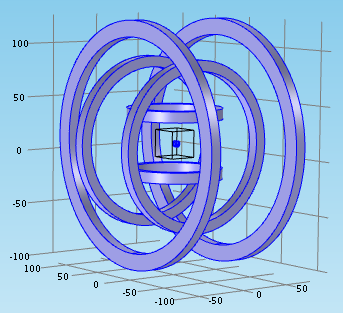
\includegraphics[width=\textwidth]{simulation}
                \caption{Simulation framework}
                \label{simulation}
        \end{subfigure}~~ 
\begin{subfigure}[b]{0.565\textwidth}
                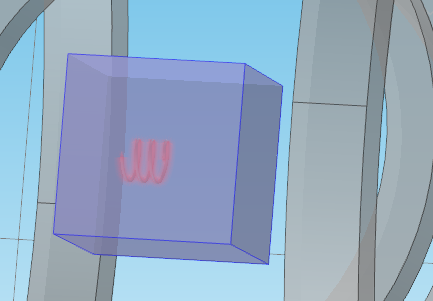
\includegraphics[width=\textwidth]{helix-in-box}
                \caption{Helix in the box}
                \label{helix-in-box}
        \end{subfigure}
      
        \caption[Simulation framework]{Simulation framework. (a) The framework consists of the three inset coils,
a fluid bux with a microhelix inside (b).}\label{Simulation framework}

   %add desired spacing between images, e. g. ~, \quad, \qquad, \hfill etc.
          %(or a blank line to force the subfigure onto a new line)
       
         %add desired spacing between images, e. g. ~, \quad, \qquad, \hfill etc.
          %(or a blank line to force the subfigure onto a new line)

\end{figure}

The effect of microhelix design parameters such as helical angle on rotational velocity of microhelix examind
under the simulation. The considered parameters are;
  
\begin{itemize}
  \item Helix angle
  \item Helix pitch
  \item Helix radius
  \item Helix filament radius
\end{itemize}

\begin{figure}
        \centering
        \begin{subfigure}[b]{0.48\textwidth}
                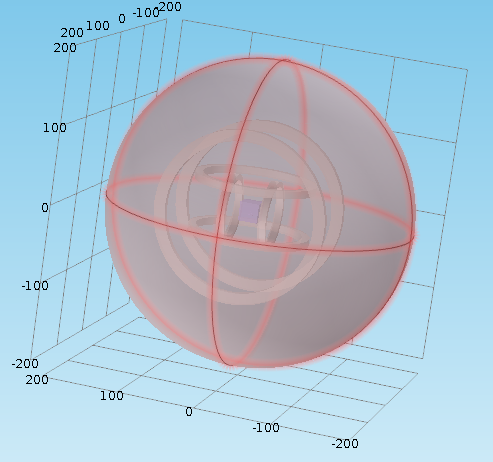
\includegraphics[width=\textwidth]{simulationDomain}
                \caption{Simulation domain}
                \label{simulation}
        \end{subfigure}~~ 
\begin{subfigure}[b]{0.48\textwidth}
                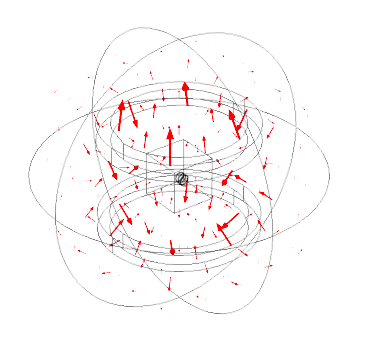
\includegraphics[width=\textwidth]{arrow_magnetic}
                \caption{Magnetic flux density}
                \label{helix-in-box}
        \end{subfigure}
      
        \caption[Simulation domain]{Simulation domain. (a) The sphere domain is defined for solving the model so the volume of
effective magnetic flux in the model can be obtained (b).}\label{Simulation domain}

   %add desired spacing between images, e. g. ~, \quad, \qquad, \hfill etc.
          %(or a blank line to force the subfigure onto a new line)
       
         %add desired spacing between images, e. g. ~, \quad, \qquad, \hfill etc.
          %(or a blank line to force the subfigure onto a new line)

\end{figure}

The result of each parameteres\rq{}s effect on the rotational velocity of the microhelix is
 presented as following. The curve in the figure \ref{RV_pitchAngle} describes the relationship between
the helical angle and rotational velocity. 
The helix with small helix angle will not result in rotating 
helix as the rotational velocity minor. 

\begin{figure}
  \centering
%\begin{wrapfigure}{r}{0.5\textwidth}
%  \begin{center}
    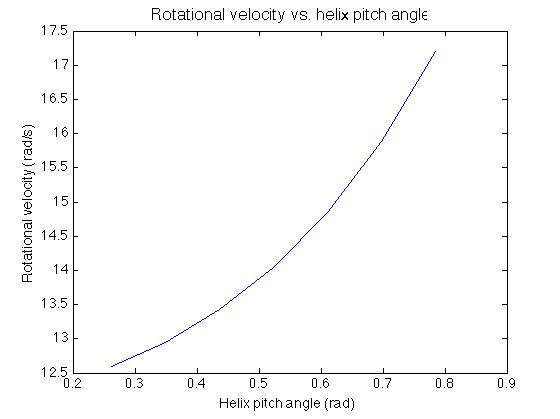
\includegraphics[width=0.80\textwidth]{RV_pitchAngle}
  \caption[Rotational velocity vs. helix angle]{Rotational velocity vs. helix angle}
  \label{RV_pitchAngle}
%\end{center}
%\end{wrapfigure}
\end{figure}





\begin{figure}
  \centering
%\begin{wrapfigure}{r}{0.5\textwidth}
%  \begin{center}
    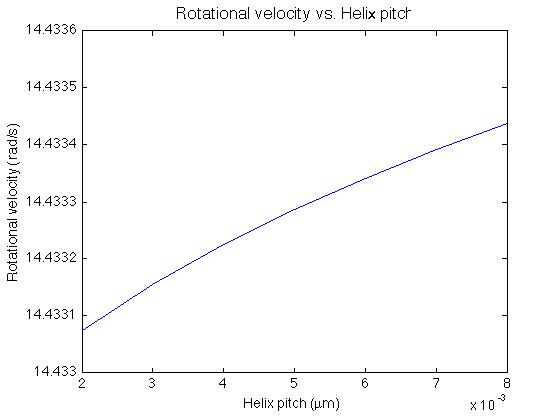
\includegraphics[width=0.80\textwidth]{RV_helixPitch}
  \caption[Rotational velocity vs. helix pitch]{Rotational velocity vs. helix pitch }
  \label{RV_helixPitch}
%\end{center}
%\end{wrapfigure}
\end{figure}

The figure \ref{RV_helixRadius1} describes the reverse relation between the helix radius and rotational
velocity. As the radius of the helix is increasing the rotational velocity is decreasing, the highest rotational
velocity is just above $14 rad/s$ for the microhelix with $2 \mu m$ radius. The similar behaviour observed
in figure \ref{RV_filamentRadius} which is dropping in rotational velocity by increasing the filament radius.
However, the range of figurs in the otational velocity axis shows the helix filament radius does not have
magnifisant effect on the rotational velocity. Whilst, the considerable changes in rotational velocity occurs
by changing the helix angle and helix radius (figurs \ref{RV_helixRadius1}, \ref{RV_pitchAngle}). 




\begin{figure}
  \centering
%\begin{wrapfigure}{r}{0.5\textwidth}
%  \begin{center}
    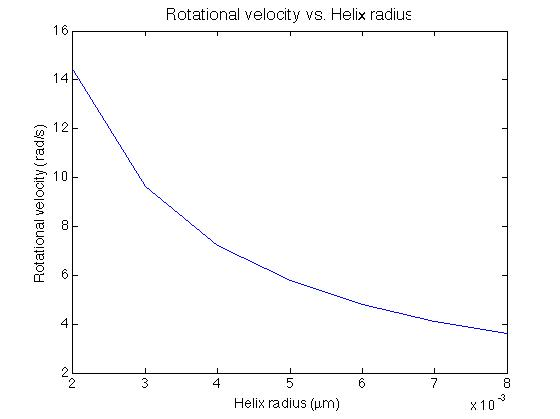
\includegraphics[width=0.90\textwidth]{RV_helixRadius1}
  \caption[Rotational velocity vs. helix rediu]{Rotational velocity vs. helix redius }
  \label{RV_helixRadius1}
%\end{center}
%\end{wrapfigure}
\end{figure}



\begin{figure}
  \centering
%\begin{wrapfigure}{r}{0.5\textwidth}
%  \begin{center}
    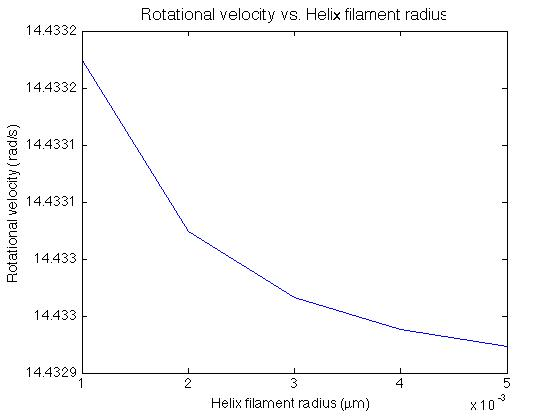
\includegraphics[width=0.90\textwidth]{RV_filamentRadius}
  \caption[Rotational velocity vs. helix filament radius]{Rotational velocity vs. helix filament radius }
  \label{RV_filamentRadius}
%\end{center}
%\end{wrapfigure}
\end{figure}

There is a linear relationship between rotational and translational velocity of microhelix as it is shown 
in figure \ref{Rotational velocity vs. translational velocity}.



\begin{figure}
  \centering
%\begin{wrapfigure}{r}{0.5\textwidth}
%  \begin{center}
    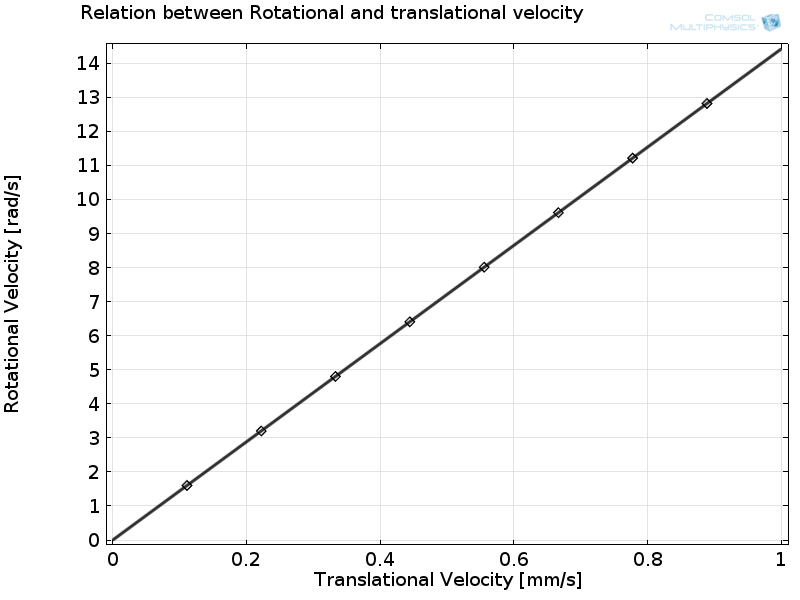
\includegraphics[width=0.80\textwidth]{Trans_Rot_}
  \caption[Rotational velocity vs. translational velocity]{Rotational velocity vs. translational velocity}
  \label{Rotational velocity vs. translational velocity}
%\end{center}
%\end{wrapfigure}
\end{figure}




%simulation result
The 


\begin{figure}
  \centering
%\begin{wrapfigure}{r}{0.5\textwidth}
%  \begin{center}
    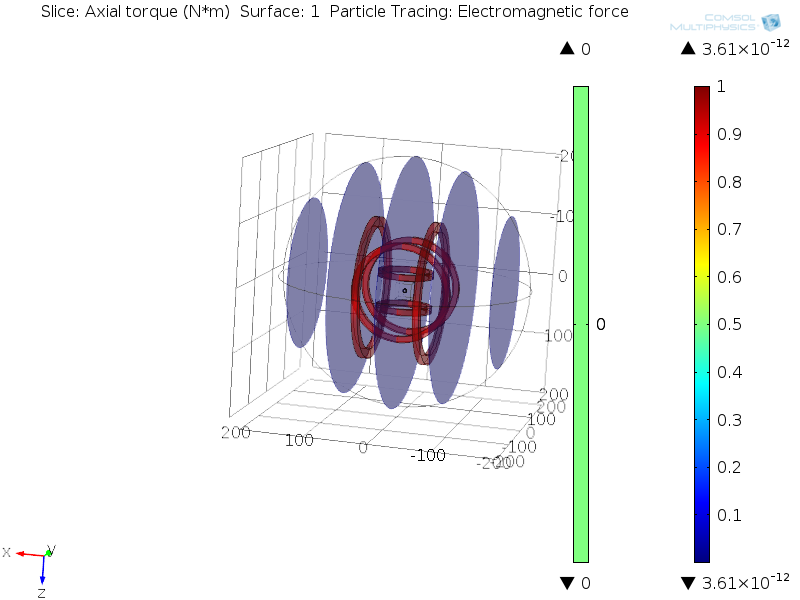
\includegraphics[width=0.80\textwidth]{force_torque}
  \caption[Rotational velocity vs. translational velocity]{Rotational velocity vs. translational velocity}
  \label{Rotational velocity vs. translational velocity}
%\end{center}
%\end{wrapfigure}
\end{figure}




\begin{figure}
  \centering
%\begin{wrapfigure}{r}{0.5\textwidth}
%  \begin{center}
    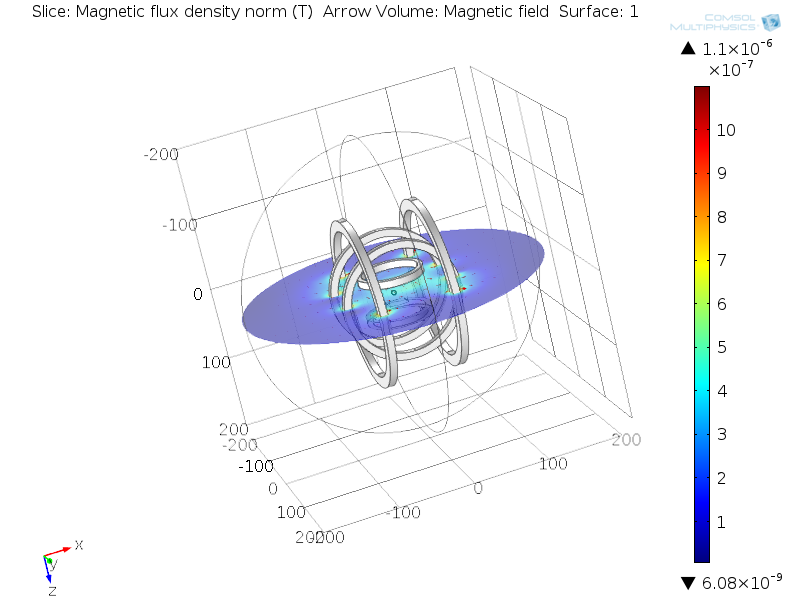
\includegraphics[width=0.80\textwidth]{magnetic_field.png}
  \caption[Rotational velocity vs. translational velocity]{Rotational velocity vs. translational velocity}
  \label{Rotational velocity vs. translational velocity}
%\end{center}
%\end{wrapfigure}
\end{figure}



\begin{figure}
  \centering
%\begin{wrapfigure}{r}{0.5\textwidth}
%  \begin{center}
    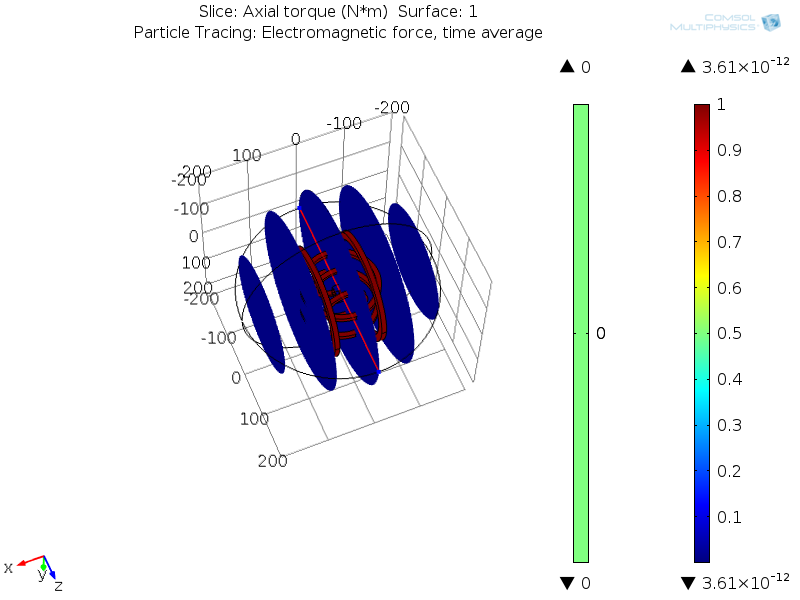
\includegraphics[width=0.80\textwidth]{moving_direction.png}
  \caption[Rotational velocity vs. translational velocity]{Rotational velocity vs. translational velocity}
  \label{Rotational velocity vs. translational velocity}
%\end{center}
%\end{wrapfigure}
\end{figure}


\section{Fabrication}

The design of the microrobot in this study is focused on the microswimmer with helical shape tail 
and a possible propeller as a head that is attached to the helix body. Therefore, after studying the 
key characteristic of the helix and identifying effective parameters a series of design were made. We started 
by reproducing the previous design that has been made by few researchers in this field and finally proposing 
new design for the helical shape microswimmers. The design software called Solidwork has been used for 
designing purpose and nanoscribe technology for the fabrication stage. In the following sections we present 
each design and the fabricated result.

\paragraph{Circle base filament}
The popular design for the helix is the one with the filament having a circle base. The design is varied in terms of 
changing the filament radius, helix pitch, helix length and helix radius. Some of the design were successfully fabricated
as it shows in the figure \ref{Circle base helix}. The figure \ref{Damaged structures} presented a faulty result which is as result of applying low power or 
high power laser beam in the fabrication process. Also another type of faulty result can be seen in the figure
which shows very small pitch length could not fabricated successfully.


\begin{figure}
        \centering
        \begin{subfigure}[b]{0.50\textwidth}
                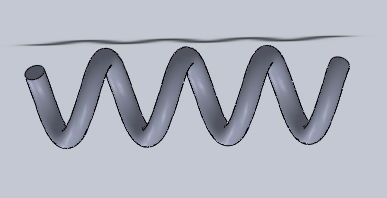
\includegraphics[width=\textwidth]{simpleHelixSolid}
                \caption{Design of circle base helix}
                \label{simpleHelixSolid}
        \end{subfigure}~
       \begin{subfigure}[b]{0.48\textwidth}
                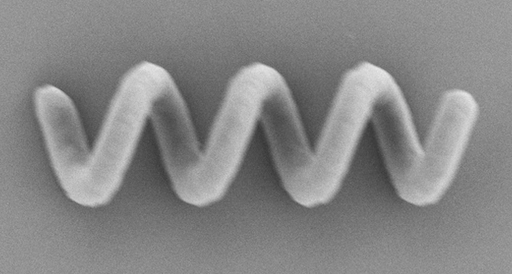
\includegraphics[width=\textwidth]{CircleBase}
                \caption{Fabricated circle base helix}
                \label{CircleBase}
        \end{subfigure}
        \caption[Circle base helix]{Circle base helix. This is the helix with $12 \mu m$  length and $4\mu m$ pitch. (a) Helix in design
stage and (b) shows the fabricated result.}\label{Circle base helix}

   %add desired spacing between images, e. g. ~, \quad, \qquad, \hfill etc.
          %(or a blank line to force the subfigure onto a new line)
       
         %add desired spacing between images, e. g. ~, \quad, \qquad, \hfill etc.
          %(or a blank line to force the subfigure onto a new line)

\end{figure}




\begin{figure}
        \centering
        \begin{subfigure}[b]{0.40\textwidth}
                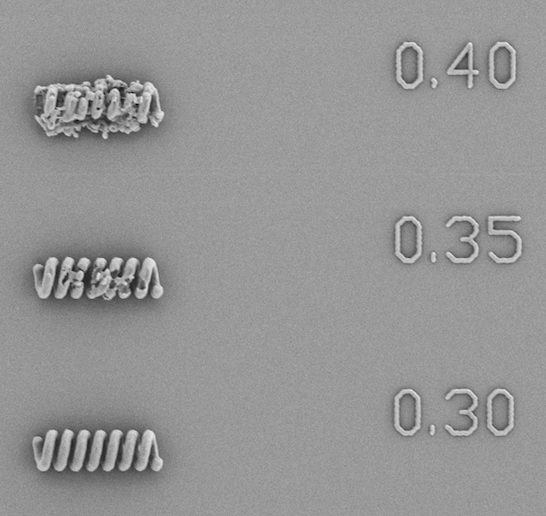
\includegraphics[width=\textwidth]{highLaser}
                \caption{Damaged structre}
                \label{Damaged structre}
        \end{subfigure}~
       \begin{subfigure}[b]{0.595\textwidth}
                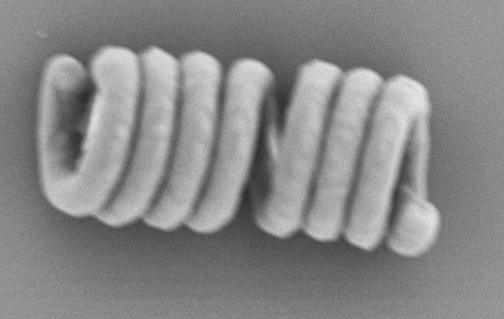
\includegraphics[width=\textwidth]{smallPitchCircle}
                \caption{Small pitch helix}
                \label{smallPitchCircle}
        \end{subfigure}

  \begin{subfigure}[b]{0.45\textwidth}
                \includegraphics[width=\textwidth]{sphereFabricated}
                \caption{Helix with a sphere head}
                \label{sphereFabricated}
        \end{subfigure}~
       \begin{subfigure}[b]{0.53\textwidth}
                \includegraphics[width=\textwidth]{largePitch}
                \caption{Large pitch helix}
                \label{largePitch}
        \end{subfigure}
        \caption[Fabricated structures]{The structure (a) is damaged as a result of high 
laser beem and structure (b) has a small pitch $1.3 \mu m$ and the result is not satisfiable. The structure
with the sphere head (c) is fabricated and the helix with the larger pitch (d) with proportion relative to
rest of helix character is clearly shown,}\label{Damaged structures}

   %add desired spacing between images, e. g. ~, \quad, \qquad, \hfill etc.
          %(or a blank line to force the subfigure onto a new line)
       
         %add desired spacing between images, e. g. ~, \quad, \qquad, \hfill etc.
          %(or a blank line to force the subfigure onto a new line)

\end{figure}



\paragraph{Rectangle base filament}

The second design has the rectangle base filament. They can make two different helix shape depends on which side of
the rectangle is revolved around the helix central axis in the design stage. The
 figure \ref{Rectangle based structures} shows a variaty of design
based on the rectangle filament with different pitch, length and helical radius.



\begin{figure}
        \centering
        \begin{subfigure}[b]{0.49\textwidth}
                \includegraphics[width=\textwidth]{Cursor}
                \caption{Small pitch rectangle base filament}
                \label{Rectangle base filament}
        \end{subfigure}~
       \begin{subfigure}[b]{0.505\textwidth}
                \includegraphics[width=\textwidth]{vertical-rentanglebased}
                \caption{Vertically fabricated ractangle based helix}
                \label{vertical-rentanglebased}
        \end{subfigure}

  \begin{subfigure}[b]{0.59\textwidth}
                \includegraphics[width=\textwidth]{ribbon}
                \caption{Rectangle based helix with large length}
                \label{ribbon}
        \end{subfigure}~
       \begin{subfigure}[b]{0.395\textwidth}
                \includegraphics[width=\textwidth]{threeHelix}
                \caption{Revolved }
                \label{threeHelix}
        \end{subfigure}

\begin{subfigure}[b]{0.50\textwidth}
                \includegraphics[width=\textwidth]{closeRectangle}
                \caption{The rectangle base}
                \label{closeRectangle}
        \end{subfigure}~
       \begin{subfigure}[b]{0.475\textwidth}
                \includegraphics[width=\textwidth]{collaps}
                \caption{Collapsed structures}
                \label{collaps}
        \end{subfigure}

        \caption[Rectangle based structures]{Rectangle based structures. The structures (a) and (b) are examples of
revolving the smaller side of the rectangle around the central axis of helix. The structure 
can printed vertically (b). The structures with small pitch (a) will not printed ideally whilst
the one with larger pitch (d) printed clearly. The printed structure can collapse (f)
and result in overlapping each other. Highly zoomed image (e) shows the rectangle base of the
helix.}\label{Rectangle based structures}

   %add desired spacing between images, e. g. ~, \quad, \qquad, \hfill etc.
          %(or a blank line to force the subfigure onto a new line)
       
         %add desired spacing between images, e. g. ~, \quad, \qquad, \hfill etc.
          %(or a blank line to force the subfigure onto a new line)

\end{figure}



\paragraph{Pitch variable helix}

In order to be able coating the structures with magnetic material, structures are preffered to printed vertically. 
The new design is made which in helix has a variable pitch. The problem with previous design was the starting helix
angle from the bottom of the helix was too high. Therefore, the structure had a poor surface to rely on that in a vertical
position. The first solution was making structures with the small helix pitch so there are stronger base for vertically
printing. However, as it is shown in the fogure \ref{collaps} part (a) the overall result of the helix with the small pitch
is not satisfiable. Thus, the idea of designing a helix with variable pitch enable us to meet both requirements. The
other advantage of having the variable pitch is providing the stonger base for the microhelix with any attached 
propeller. The result of the new design is shown in figure \ref{Pitch variable}.



\begin{figure}
        \centering

  \begin{subfigure}[b]{0.566\textwidth}
                \includegraphics[width=\textwidth]{constant-pitch}
                \caption{Constant pitch helix}
                \label{constant-pitch}
        \end{subfigure}~
  \begin{subfigure}[b]{0.42\textwidth}
                \includegraphics[width=\textwidth]{variable-pitch1}
                \caption{Variable pitch helix. }
                \label{variable-pitch1}
        \end{subfigure}
      
        \caption[Variable pitch helix]{Variable pitch helix. The image (a) is shown the constant pitch helix which could not printed
vertically. However, the image (b) represents the successful vertically fabricated of (a) by making its pitch
variable.}\label{Pitch variable}

   %add desired spacing between images, e. g. ~, \quad, \qquad, \hfill etc.
          %(or a blank line to force the subfigure onto a new line)
       
         %add desired spacing between images, e. g. ~, \quad, \qquad, \hfill etc.
          %(or a blank line to force the subfigure onto a new line)

\end{figure}



%%%%%%%%%
%%%%%%%%%%%%%%%%%%%% Discussion %%%%%%%%%%%%%
%%%%%%%%%
\chapter{Discussion}\label{discussion}

\paragraph{}
The design of microhelix is based on the key characteristics of the helical shape. A filament base of a 
popular helix has a circle shape. Therefore, the initial design was the helix with a circle base filament and then
 it integrated with different propeller head such as a sphere and a square. Changing each character at a time and 
keeping the rest of characters constant optimised characteristics of microhelix. This algorithmic process was repeated
 for any new design such as helix with a rectangle base filament. The helix design should be optimised
 in terms of both fabrication and simulation.


In the fabrication process, the nanoscribe technology used for 3D printed in micro size. This
 technology is based on lithography system to write microstructure. The result of fabricated structures
 showed the required laser power is varies to write each microhelix design. The result of horizontally printing 
microhelix was successful in many cases. However, few cases destroyed either because of applying high laser 
power or under power. The amount of appropriate laser power was design dependent and couldn\rq{}t generalise for 
all the design. A number of few cases were collapsed only during developing process. The vertically fabricating 
microhelix was a challenge, as most of the design did not provide sufficient contact surface to support their 
weight. The new helix design with a variable pitch made the structures with sufficient contact area with the
 substrate. The variable pitch helix has the smaller pitch in the bottom and larger pith on the rest of the 
body. As a result small pitch in a bottom satisfies the vertically fabricated requirement of microhelix 
and larger pitch on the rest of the helix body helps the swimming motion of microhelix. 

\paragraph{}

To model the swimming motion of the microhelix three models were studied and \ac*{RFT} were
 implemented in the simulator. \ac*{RFT} has ignored the 
hydrodynamic interaction between the fluid flow produced by different segment of the microhelix. 
Therefore, in the microhelix with the smaller pitch the interaction between various part of the helix
 increased and the helix will convert to the cylinder. This issue might result in a failure for predicting
 the force and torque in microhelix with incredible small pitch. Thus, the variable pitch microhelix will help to avoid that issue.  

To model the swimming motion of the microhelix three models were studied and \ac*{RFT} were
 implemented in the simulator. 
Each microhelix propulsion model was segmented the filament of a 
microhelix differently. Then the model analyses an interaction of a small segment of
 filament with hydrodynamic of a high viscous fluid to achieve non fluidic force, torque and drag 
acts on a helix body. All three propulsion models apply on the microhelix with the circle base 
filament. Therefore, we will not be able to implement the propulsion model for other designs such 
as microhelix with a rectangle base filament.   




\paragraph{}

Magnetic field is a safe power source to be used for actuating microrobot in the fluidic environment. 
There are advantages to apply torque driven magnetic field over force driven which makes it preferable
 approach. Torque driven method can be applied on either microrobot with the flexible tail or a rigid 
tail. The method is more efficient than force driven as the rotation of helix leads to translational 
movement in the fluidic environment whilst the force driven method pulls the helix to generate
 the translational velocity. 

\paragraph{}

Implementing the model using simulation software is a challenge. There are not enough simulation 
software provide all the requirements of the model. Therefore modelling the simulator for microrobot
 navigation becomes more complex. For example the hydrodynamics property of the fluid and its 
effect on the swimming microrohelix cannot be modelled entirely with Matlab. COMSOL software 
is more advanced simulation in terms of solving the multiphysics model by coupling the different 
physics. However, the modelling can be performed differently by coupling different components 
of the system and occasionally the simulation result is not consistent.  












%%%%%%%%%
%%%%%%%%%%%%%%%%%%%% Conclusion %%%%%%%%%%%%%
%%%%%%%%%
\chapter{Conclusion and future work}

The magnetically actuated helical shape microrobot  has an advantage of using in vivo or in 
vitro application. The different design of microhelix has been made; some of designs were 
reproduced from previous researchers and also new design was presented. The new design 
is a helix with a variable pitch that makes the structure enables to stand vertically during fabrication 
process. 
The other advantage of the new design is providing the stronger base for the structure for the case
 of having microrbot with attached propeller. The \ac*{RFT} used as a locomotion model for simulating 
microrbot motion. Other propulsion models presented are \ac*{SBT} and \ac*{RSM} to describe the 
motion of microhelix. In terms of design, helix angle is the most effective character of the helix that has 
an effect on its swimming efficiency. The other characteristic such as helix radius has a smaller effect. 
The fabrication process performed by nanoscribe facility and microstructures were observed 
under \ac*{SEM}. 
Initially Matlab used for implementing the model and towards the end of the project the 
COMSOL Multiphysics software used because of limitation of Matlab to solve the model.  



\paragraph{Future work}
In order to validate the result of this study we need to run an experiment in a laboratory 
to compare the result of the simulation with the experiment. The simulation framework is
 required optimisation in order to simulate microhelix in fluids with different viscosity. In terms 
of fabrication, the effects of using combination of magnetic material for microhelix coating can
 be analysed. The ideal locomotion method for microrobot is still required more investigation. 


The possibility of actuating a microrobot with other power source such as ultrasonic can be
 considered. The fundamental design of mcirorobot can be integrated with other tools to build 
an advanced microrobot. The design of an advanced microrobot is an application dependent. 
The microhelix with its transport claw is already proposed and demonstrated their result to move 
micro objects. Therefore, researching on current medical application and limitation of the surgical
 tools can lead to design an advanced microrobot for a specific application. The swarms of 
microrobot and a mechanism for control them individually will improve their performance.      










%%%%%%%%%%%%%%%%% List of the references are not used directly in the text %%%%%%% 
\nocite{lauga2006swimming}

%%%%%%%%%%%%%%


%\renewcommand{\bibname}{References}
\bibliographystyle{unsrtnat}
%\bibliographystyle{plainnat}
\bibliography{References} 
%\addcontentsline{toc}{chapter}{\numberline{}References}

\end{document}